\chapter{\label{chap:trainingExperiment}Training Experiment}

\minitoc


\section{Abstract}
This study employed a controlled experimental environment to further test an hypothesised relationship between joint action, team click, and social bonding.  The core prediction of this dissertation, that athletes who perceived higher quality team performance in joint action would also experience higher levels of team click and social bonding, was partly confirmed in an \textit{in situ} survey study (Chapter 8 HYPERLINK). The causal mechanisms and system dynamics underlying this relationship remain unknown.

In the present study, 58 Professional Chinese rugby players (Men = 31) participated in a between-subjects design in which athletes' expectations for joint action training drill \citep[``Invasion drill''][]{Passos2011}) were manipulated in one of two conditions.  Athletes in the ``low difficulty'' condition were primed with information to suggest that the training drill would require minimal rugby-specific individual and joint-action competence (i.e., 2/10 difficulty rating).  By contrast, in the ``high difficulty'' condition, athletes were primed to expect the training drill to be relatively difficult (8/10 difficulty rating). Pre- and post-experiment surveys were conducted, measuring athletes' perceptions of main variables of interest (individual and group performance, team click, and social bonding (both to the training group and the team more generally)), as well as athlete personality type and states of athlete states of arousal, fatigue, and injury.  Video footage of each experimental session was also recorded to derive an objective measure of interpersonal coordination not reliant on self-report. It was predicted that athletes in the ``high-difficulty'' condition would experience higher levels of team click and social bonding due to more positive perceptions of group performance relative to prior expectations .  Athletes in the ``low difficulty'' condition would on average experience less strongly the ``click'' of joint action and social bonding because they would not experience the same level of positive violations of expectations around group performance.  Results provided some confirmation of these predictions.

%Video footage was analysed for evidence of dynamic coupling between co-actors as well as defenders \citep{Schmidt2011,Richardson2012,Passos2012}, and these data were compared to psychological measures in order to explore psychological correlates of effective  interpersonal movement coordination in joint action.

%for two reasons: 1) athletes with expectations of higher difficulty would pay greater attention to coordinating action with others, and
%


\section{Introduction}
The phenomenon of ``click'' in joint action is widely substantiated by intuition and anecdote in group activities spanning sport to music/dance and even interactions in sedentary work place contexts.  The cognition of team click and its social effects remain poorly understood, however.  In this dissertation, I pursue the theory that team click in joint action could be an important causal explanation for the relationship between group exercise and social cohesion.

The previous chapter presented empirical evidence of a relationship between perceptions of joint action success and social bonding, fully mediated by the phenomenon of team click.  The results of this naturalistic \textit{in situ} study are noteworthy as they provide evidence for the prediction that perceptions of joint action influence psychological processes of affiliation and connection with teammates, possibly via the mediating construct of team click.  A high stakes rugby tournament, however, contains many variables that may have confounded the specific relationships that are of interest in this dissertation. In a high stakes Tournament, athletes are provided with explicit feedback about joint action (in the form of winning and losing each game, for example), and there are many other dimensions to rugby that could have been driving social bonding effects, such as the extremely high levels of physiological exertion and body-on-body contact associated with rugby games.  Although some of these factors were addressed through statistical controls, these controls were based largely on athlete self-report and indirect measures of athlete experience (such as objective measures of performance).  Controlled experimental research is needed in order to more directly access causal mechanisms that underpin the relationship between joint action and social bonding.

Existing theory suggests that positive violation of expectation around joint action could be the source of feelings of team click and social bonding. How is it possible to experimentally manipulate conditions conducive to maximising this dimension of joint action? In addition, how is it possible to isolate joint action from other potential sources of information regarding the team and its performance such as explicit feedback from coaches and other players surrounding performance and joint action outcome? This experimental study was designed with these considerations in mind.


%A relationship between violation of expectations surrounding team performance and feelings of team click was also observed, but a model of the relationship between team performance expectation and social bonding did not reliably fit the data.

The Lit Review (unfinished):
1. Re-cap literature (Synchrony, joint action, pink noise, team click)
2. Extend to predictive coding in joint action
3.Priming literature: prime difficulty and uncertainty:
Solution: manipulate the level of uncertainty of information regarding the expectation.


%Immediately after the opening comes the literature review, which describes relevant previous research on the topic and can be anywhere from several paragraphs to several pages in length. However, the literature review is not simply a list of past studies. Instead, it constitutes a kind of argument for why the research question is worth addressing.

%By the end of the literature review, readers should be convinced that the research question makes sense and that the present study is a logical next step in the ongoing research process.   it is extremely important to start with an outline of the main points that you want to make, organized in the order that you want to make them. Or if you are proposing a new theory, then of course you should discuss findings that are consistent with that theory. However, if there are other findings that are inconsistent with it, again, you should discuss them too.


These considerations lead to the hypothesis that expectations of higher levels of technical challenge in joint action will lead to higher levels of social bonding, due to the likelihood that athletes will experience more positive violations of expectations around team performance in the high-difficulty prime than in a low difficulty prime. It was predicted that the feeling of team click would mediate a relationship between positive violations of expectations and social bonding.  The predictions are outlined as follows:

\begin{description}
\item[Prediction 1:] More positive perceptions of team performance relative to prior expectations will correlate with higher feelings of team click with the training group
\item[Prediction 1.a:] Violations of expectations around team performance moderate the relationship between perceptions of joint action success and team click training group
\item[Prediction 2:] Feelings of group click will positively correlate with feelings of social bonding to the group
\item[Prediction 3:] More positive perceptions of team performance relative to prior expectations will predict higher levels of social bonding to the training group
\item[Prediction 4:] Feelings of group click will mediate a relationship between more perceptions of group performance relative to prior expectations and social bonding to the group
\end{description}

A between-subjects experimental design was used, in which expectations of technical difficulty was manipulated in one of two conditions, ``high difficulty'' and ``low difficulty'' condition.  Surveys measuring athletes' perceptions of performance in joint aciton relative to prior expectations, feelings of team click, and feelings of social bonding to the specific training group were recorded both before and after the experiment.

%The closing of the introduction—typically the final paragraph or two—usually includes two important elements. The first is a clear statement of the main research question or hypothesis. This statement tends to be more formal and precise than in the opening and is often expressed in terms of operational definitions of the key variables. The second is a brief overview of the method and some comment on its appropriateness.

%These considerations lead to the hypothesis that the more bystanders to an emergency, the less likely, or the more slowly, any one bystander will intervene to provide aid. To test this proposition it would be necessary to create a situation in which a realistic “emergency” could plausibly occur. Each subject should also be blocked from communicating with others to prevent his getting information about their behavior during the emergency. Finally, the experimental situation should allow for the assessment of the speed and frequency of the subjects’ reaction to the emergency. The experiment reported below attempted to fulfill these conditions (p. 378).

%\subsection{Design}
%The design of a study is its overall structure. What were the independent and dependent variables? Was the independent variable manipulated, and if so, was it manipulated between or within subjects? How were the variables operationally defined?

\section{Method}



\subsection{Participants}
64 professional Chinese rugby players from two provincial programs were recruited for the study (men = 32, M(age) = 21.33 SD = 3.33, range = 16-29).  Athletes were recruited from two provincial rugby programs, 32
participants were athletes from Shandong province (men = 15, M(age) = 22.1) and the remaining 32 athletes were from Beijing province (men = 16, M(age) = 20.4).  This study was approved by the University of Oxford’s Central University Research Ethics Committee (SAME/CUREC1A/15-059).


\subsection{Materials}


\begin{figure}[htbp]
  \centering
      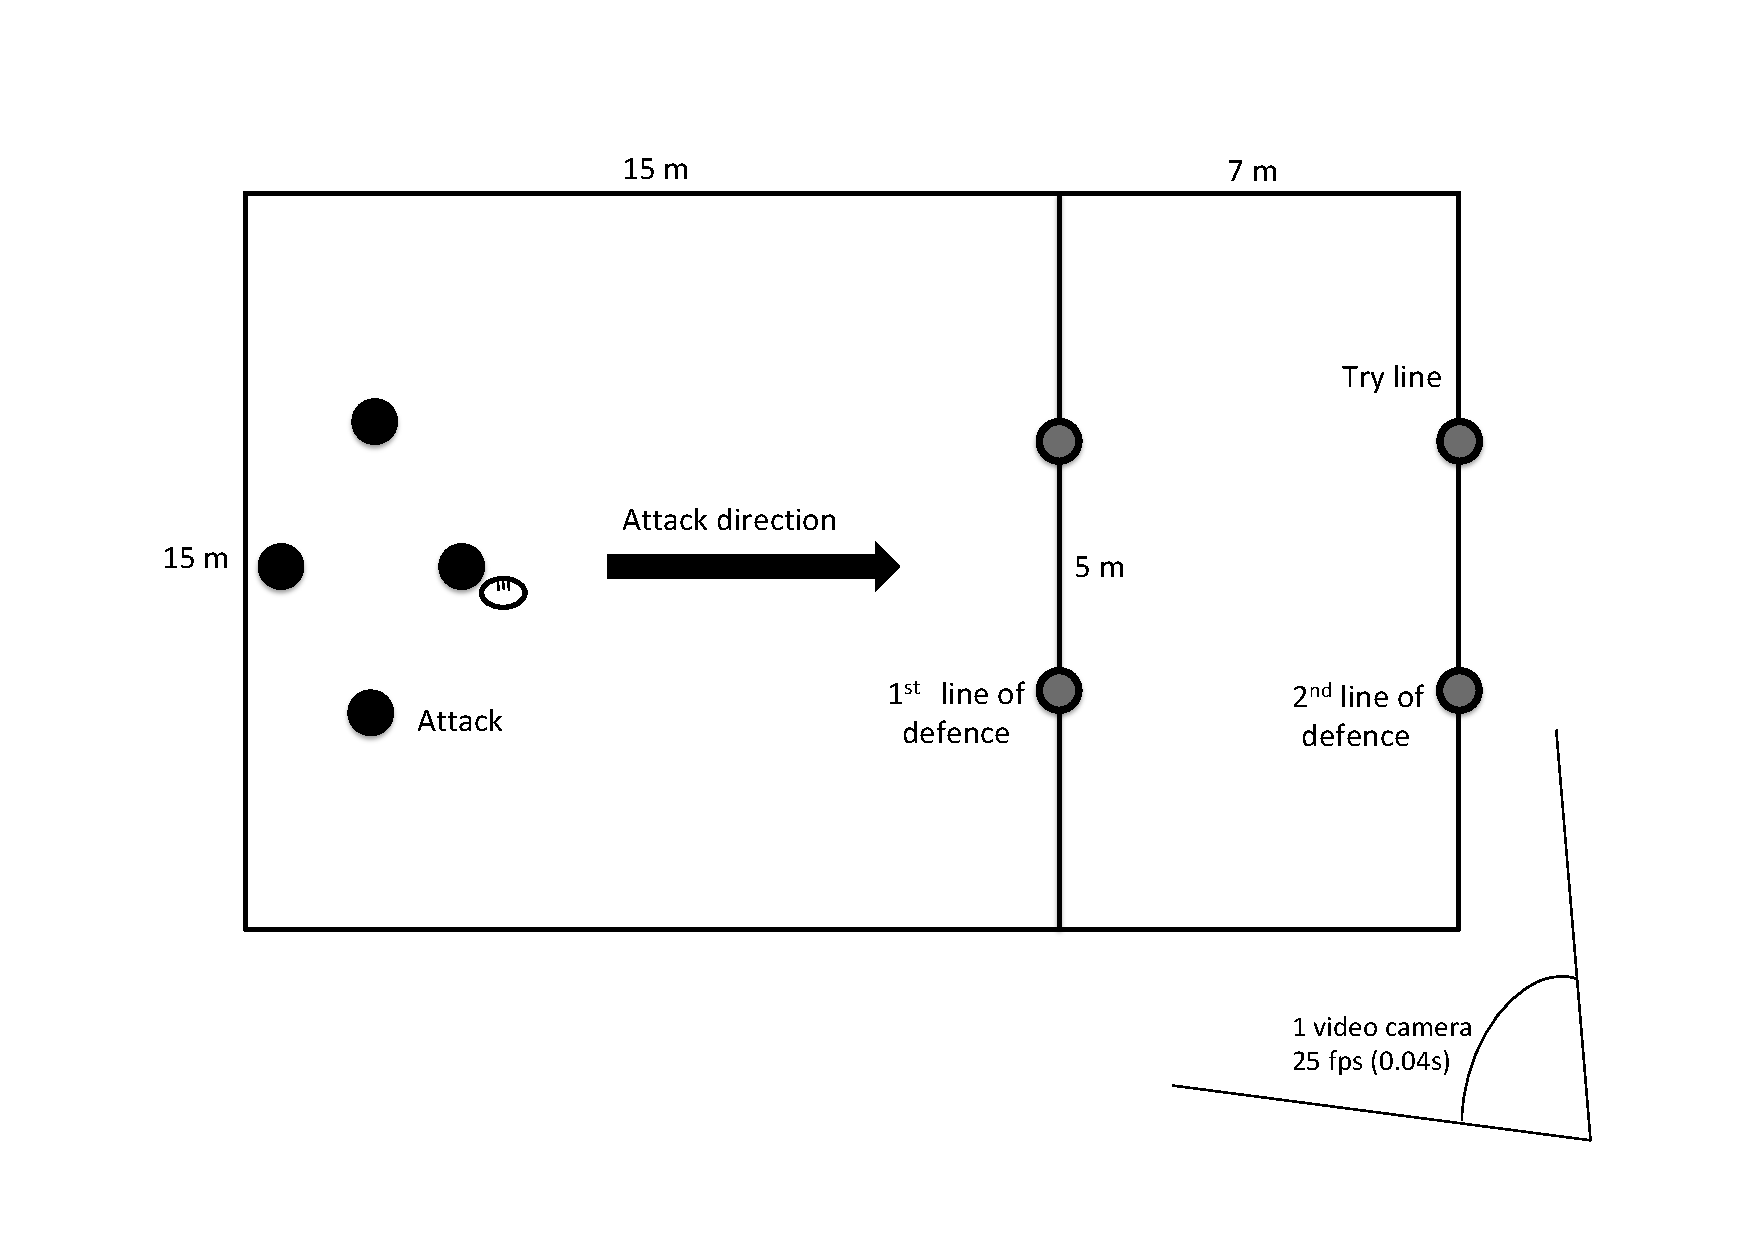
\includegraphics[width=0.9\linewidth,keepaspectratio] {images/invasionDrill}
      \caption{The Invasion Drill, adapted from Passos (2011)}
      \label{fig:invasionDrill}
  \end{figure}


\subsubsection{Experimental Paradigm: Invasion Drill}
This study required athletes to participate in a common rugby training drill, which was preceded by one of two experimental primes—--a ``high difficulty'' condition, or a ``low difficulty'' condition.   Replicating \textcite{Passos2011}, a common training drill known as ``invasion drill'' \citep{Biscombe1998} was selected as it was representative of a typical subphase of joint action in rugby union.
In this drill, a group of four rugby players form an attacking group and two pairs of opponents form a first and second defensive line.  There were two performance aims of this drill: (a) attackers were asked carry the ball into the try area, and (b) defenders were asked to stop the attacker’s progression toward the try line.
One trial consisted of one attempt by the attacking sub-group to penetrate two defending sub-groups, and carry the ball over the try line. The drill was conducted on a regulation multipurpose 110m x 70m grass or artificial turf training field within a 22m x 15m rectangle area marked by plastic cones (see Figure ~\ref{fig:invasionDrill}). The ball used was size 5, as recommended by World Rugby for this age group of athletes.


%The training drill, known as ``invasion drill,'' requires eight athletes, one sub-grouof four attackers and two sub-groups of two defenders.  The primary aim of the drill is for the sub-group of 4 attacking players to successfully penetrate two consecutive lines of two defenders (also commonly known as a ``4 on 2 + 2'' drill). The aim of the two defending sub-groups is to stop the attacking team from achieving the primary goal, by interfering with their coordination by halting the ball-carrier, or the ball in flight between attacking players.


\subsubsection{Experimental Conditions: high and low difficulty}
Two different pre-experiment primes were developed for the same training drill in order to manipulate athletes’ expectations around the technical difficulty of the impending joint-action task.  Athletes in the ``high difficulty'' condition learned that the overall average difficulty rating for the training drill, provided by World Rugby coaches and athletes, was 77.5/100, or approximately 8 out of 10.  Athletes were told that the drill would require an extension of their abilities as individuals and as a training group.  Athletes in the ``low difficulty'' condition, by contrast, learned that they would be participating in an ostensibly different drill with an overall average difficulty rating (provided by World Rugby coaches and athletes) of 22.5/100, or approximately 2 out of 10 (see Appendix ~\ref{app6:trainingExperiment} Sections ~\ref{app6:conditionPrime}\nobreakdash~\ref{app6:conditionPrimeLow} for full script). In reality, the training drill was exactly the same for each experimental session, and the relative difficulty of this drill was estimated in a pilot study to be approximately 5/10, see Appendix ~\ref{app6:trainingExperiment} Section ~\ref{app6:difficultyPilot} for full explanation of pilot study).  The experiment primes were designed to encourage athletes to either over or under rate the difficulty of the impending training drill. If successful, the prime would alter athletes' expectations around certainty of performance, such that athletes in the high difficulty condition would enter the training drill with expectations for performance that were on average lower than athletes in the low difficulty prime. In turn, athletes in the high difficulty condition would experience more positive perceptions of resulting group performance relative to prior expectations.  Athletes in the low difficulty, by contrast, would on average experience experience less positive violations of expectations around group performance.  Surveys were designed and administered using Qualtrics software (Qualtrics version 9, Provo, UT). Survey data were processed and analysed using the R environment (R Development Core Team, 2006).


\subsubsection{Measures}


    % latex table generated in R 3.5.0 by xtable 1.8-2 package
% Mon Aug 27 19:27:18 2018
\begin{table}[ht]
\centering
\begin{tabular}{llccc}
  \hline
 & Items & Baseline & Pre & Post \\ 
  \hline
1 & Performance(Team) & * &  &  \\ 
  2 & TeamClick(Team) & * &  & * \\ 
  3 & SocialBonding(Team) & * &  & * \\ 
  4 & Performance(Group) &  & * & * \\ 
  5 & TeamClick(Group) &  & * & * \\ 
  6 & SocialBonding(Group) &  & * & * \\ 
  7 & Performance(Ind) & * & * & * \\ 
  8 & Arousal &  & * & * \\ 
  9 & Exertion &  &  & * \\ 
   \hline
\end{tabular}
\caption{Survey items measured at each time point} 
\label{tab:surveyItemsByTime}
\end{table}



\myparagraph{Surveys}
Surveys were administered at three time points:

\begin{enumerate}
  \item Baseline: approximately 24 hours before the experiment
  \item Pre-Experiment: immediately before the experiment after receiving the experimental prime.
  \item Post-Experiment: once immediately following the completion of the experiment (Post-Experiment)(see ~\ref{tab:surveyItemsByTime}).
\end{enumerate}

Consistent with the previous study (Chapter 8), athletes responded to questions about:

\begin{enumerate}
  \item Performance: perceptions of components and overall individual and team performance in joint action,
  \item Team Click: feelings associated with team click in joint action, and
  \item Social Bonding: feelings of social bonding and group membership.
  \item Moderator Variables: Injury, arousal, fatigue, personality type, etc.
\end{enumerate}

\myparagraph{Baseline}
At Baseline, athletes were asked about their impressions of recent individual performance and the performance of their province team as a whole.  Survey items included questions relating to specific components of on-field performance (e.g., team components: Attack, defence, on-field communication, and support play; individual components: Passing technique, one-on-one tackling, effectiveness in contact areas) as well as items relating to overall impressions of performance, for example: ``How well do you feel your team has been performing in training and competition over the past month?'' (100 point scale, 0 = ``Extremely bad'', 100 = ``Extremely good'').  Athletes also responded to questions about feelings of team click and social bonding with their team as a whole. In addition, the Baseline survey also included items concerning basic personal information, current injury status, subjective and objective measures of technical competence, and personality type.  For a full explanation of survey items measured at Baseline, see Appendix ~\ref{app6:trainingExperiment} Section ~\ref{app6:surveyItemsBaseline}.


\myparagraph{Pre-Experiment}
Immediately before each experiment session, athletes were asked questions about feelings and expectations concerning their individual performance and the performance of their specific training group in the impending training drill.  For example,  athletes were asked ``How do you feel \textit{right now} about your individual performance (100 point scale, 0 = ``Extremely bad'', 100 = ``Extremely good'')''.  Athletes were also asked a series of questions about feelings of team click and social bonding to their specific training group. For team click, for example, athletes were asked questions like: ``How do you feel the tacit understanding is between the training group today?'' (100 point scale, 0 = ``Extremely bad'', 100 = ``Extremely good'').  For social bonding, athletes were asked questions like: ``How emotionally supportive does your training group feel right now?'' (100 point scale, 0 = ``Extremely weak'', 100 = ``Extremely strong'').  Questions regarding team click within each training group will from this point on be referred to as ``group click,'' and social bonding to the training group will be referred to as ``group bonding.'' For a full explanation of survey items measured at Pre-Experiment, see Appendix ~\ref{app6:trainingExperiment} Section ~\ref{app6:surveyItemsPre}.

\myparagraph{Post-Experiment}
At time 3, immediately after the completion of the experiment (Post-Experiment), athletes completed questions concerning their impression of their own performance and the performance of their training group in the training drill, relative to their prior expectations.  Athletes were also asked about their feelings group click and group bonding, as well as social bonding to the provincial team as a whole (team-focussed questions were replications of the survey items that were asked one day earlier at Baseline).  For a full explanation of Post-Experiment survey items, see Appendix ~\ref{app6:trainingExperiment} Section ~\ref{app6:surveyItemsPost}.
%~\ref{} Section ~\ref{}.

Surveys were generated in English by the researcher using Qualtrics software (Qualtrics version 9, Provo, UT). Surveys were translated into modern Chinese and back translated by two independent native Chinese speaking translators from Beijing Sports University to verify accuracy.  Athletes completed the modern Chinese version of each survey using WeChat on their personal mobile devices connected remotely to the internet.


\subsubsection{Video analysis of training group performance in training drill}
In order to produce quantitative measures of interpersonal coordination between co-actors, athletes’ motion was captured by a single digital video camera (Sony FDR-AX700 4K HDR Camcorder) mounted on a 1.2m high tripod. Digital video images of action were acquired by a computer, using a USB2.0 cable, and files were saved on an encrypted external hard disk in .AVI format.
%For image treatment, TACTO 8.0 software was used for digitising at 25 frames per second.

A research assistant (who was hypothesis bliind) analysed video footage from all 8 experiment sessions.  Each experimental trial of the Invasion Drill (16 in total) was coded according to the quality of performance relative to the primary (attacking) goal of the drill, i.e., scoring a try by carrying the ball over the try line.  A maximum value of 6 was awarded to a ``clear try'' (trials in which a clear unobstructed try was scored by the attacking sub-unit); 5 to a ``rough try'' (the ball-carrier crossed the try-line following some minimal level of physical contact or obstruction from the defence that did not halt the momentum of the attacking phase); 4 to an ``Obstructed try'' (a trial in which a try is scored, but the momentum of the attacking sub-unit was clearly interrupted); 3 to a ``no try - defence''  (a trial in which a ball carrier is completely obstructed by a defender, and the trial is unsuccessful largely due to the effectiveness of the defence); 2 to a ``no try - defence forced error'' (unsuccessful trial due to a combination of the defence and error in attack); 1 to a ``no try - unforced error'' (a failed trial due to an unforced error in attack).  For each experiment session, an average performance outcome (``Trial Outcome Average'') and the standard deviation of this mean outcome (``Trial Outcome SD'') was calculated in order to capture the central tendency and variability of performance for each training group.


\subsection{Procedure}
Permission to run the study was sought from the head coach of each of the four teams (Beijing men's, Beijing women's, Shandong men's, Shandong women's).  These coaches nominated athletes who were fit and able to complete the session without compromising their existing training schedules.  Athletes were randomly assigned to one of two conditions, and then athletes in each experimental group were subsequently adjusted subsequently so that each condition was matched as much as possible according to average training age. Once athletes were assigned to an experimental group, they were then added to a WeChat group populated by other training group members and the researcher.

\subsubsection{Cover Story}
Athletes were notified (first via WeChat and then in a team meeting) that they were participating in a trial of a number of different rugby training drills selected from a recent report by World Rugby concerning training methods for rugby sevens.  Athletes were told that the training drills had been previously rated by a selection of international level coaches and players from all over the world (including Asia and China).  Athletes were informed that the purpose of the exercise was for me to assess the ratings provided by World Rugby by replicating these drills with more rugby athletes in China.  Athletes were told that survey measures and video footage would be collected, which would be later analysed to assess individual performance of athletes in each training drill.  It was also explained to athletes that there would be a second round of drills also requiring groups of eight athletes, but the makeup of these groups may reshuffle depending on athletes preferences.  This detail allowed for the inclusion of a post-Experiment bonding measure, in which athletes were asked to what extent they wished to continue to train with the same 8-athlete team in a subsequent round of drills.

Approximately 24 hours before the experiment session, athletes were instructed to complete the baseline survey by opening a link provided in the WeChat group.  This survey included written consent for the study. Approximately 1 hour before the experiment was due to take place, athletes were administered with an experimental prime via WeChat.  In the ``high difficulty'' condition, athletes were primed to believe that they were about to participate in a very difficult training drill (on the upper end of their individual and group technical abilities), whereas athletes in the ``low difficulty'' condition were primed to believe that they were about to participate in a relatively easy training drill well within their technical abilities.  All athletes were lead to believe that athletes in the other experiment groups were performing different drills to their assigned drill. In reality, the training drill for each condition was identical, the only thing that varied was the pre-experiment prime.

Once athletes were assembled at the designated training field, I verbally re-administered the same prime that had been sent to athletes via WeChat an hour earlier.  In addition, athletes were told in more detail about the requirements of the Invasion Drill.  Specifically, athletes were told that their performance in the experiment would be assessed based on subsequent video analysis.  I told athletes that they would be assessed based on their performance in attack, defence, and their ability to coordinate attack and defence with others.  Athletes were provided with no other explicit information regarding performance goals, besides completing the experimental drill to the best of their ability within the rules of rugby.

Athletes were then administered with the time 2 survey (Pre-Experiment), which took approximately 3-5 minutes to complete.  After every athlete had finished the survey, athletes participated in a standard warm up routine lasting approximately 10 minutes, including slow jogging and dynamic stretching.  Athletes were instructed not to use the rugby ball during this period, which served to reduce the amount of incidental coordination and interaction between participants prior to the start of the experiment trials.  Once athletes had completed the warm up, the researcher assembled the group within the training drill area.  One athlete was randomly assigned to stand at each of 8 available plastic markers (6 in the case of the modified drills).  In this position, athletes were told once more about the structure and procedure for the training drill, in particular the way in which athletes were expected to rotate clockwise after every trial of the drill so that athletes did not habituate to certain positions or sub-units in the drill.

To begin the drill, the ball-carrier at the front and centre of the attack sub-group was instructed to tap the ball with his / her foot, before initiating the attacking sub-phase by advancing forward towards the defence sub-units.  In the case that the ball was immediately fumbled during the initiation of the trial, the training group was instructed to restart that trial and the trial in which the mistake was made was not counted.  Following a block of 4 practice trials, athletes were told by the researcher that the formal test was beginning.  The group of athletes then completed 16 trials of the drill, which allowed each athlete to complete four trials of attack and four trials of defence, in different positions.  Following completion of all 16 test trials, athletes were assembled by the researcher and thanked for their participation, before being sent to the sideline of the training field to complete the final post-experiment survey using their mobile devices.  Following the completion of this final survey, athletes were told that they would be informed within two days about the next experiment trial (in fact, no more experiments were taking place).

\myparagraph{Video Analysis Procedure}
The digital camera and tripod were positioned on a platform 2m above the level of the playing field, approximately 10-15m from the bottom try-line corner of the Invasion Drill perimeter (see figure ~\ref{fig:invasionDrill}).  The experimenter began video recording before the athletes arrived, and ceased recording after all athletes had left the training field following the experiment.  Digital video images of action were acquired by a computer, using a USB2.0 cable, and files were saved on an encrypted external hard disk in .AVI format.

%For image treatment, TACTO 8.0 software was used for digitizing at 25 frames per second.
%The procedure is how the study was carried out. It often works well to describe the procedure in terms of what the participants did rather than what the researchers did. For example, the participants gave their informed consent, read a set of instructions, completed a block of four practice trials, completed a block of 20 test trials, completed two questionnaires, and were debriefed and excused.


\section{Results}




\subsection{Descriptive Statistics \label{sec:descriptives}}

\subsubsection{Participants}

A total of 58 athletes ($men = 31, M(age) = 21.33 SD = 3.33, range = 16-29$) participated in eight experimental sessions. 31 participants were athletes from Shandong province ($men = 15, M(age) = 22.1$) and the remaining 27 athletes were from Beijing province ($men = 16, M(age) = 20.4$).  In one session (Shandong men's high difficulty condition) a research assistant stood in as a dummy participant for an athlete could not participate due to injury.  In the two sessions with Beijing women's team, due to failure of athletes to take part due to injury (3) or illness (2), the training drill was modified to a ``3 on 2 + 1'' drill, requiring only six athletes to complete instead of eight. In one of these experimental sessions, a female dummy participant was also required to fill in to make up a total of 6 athletes for the modified drill.  In both cases, dummy participants were competent ex-athletes who were naive to the predictions of the study.  Dummy participants did not participate in the survey responses before or after the session. Survey and video data of the remaining 58 participants was analysed.

% latex table generated in R 3.5.0 by xtable 1.8-2 package
% Wed May 16 15:48:41 2018
\begin{table}[ht]
\centering
\begin{tabular}{rlll}
  \hline
 & Overall & high & low \\ 
  \hline
n &    58 &    29 &    29 \\ 
  Age (mean (sd)) & 21.33 (3.33) & 20.48 (3.11) & 22.14 (3.39) \\ 
  Sex = male (\%) &    31 (53.4)  &    15 (51.7)  &    16 (55.2)  \\ 
  \textbf{Team} (\%) &     &     &     \\ 
     Beijing Men &    16 (27.6)  &     8 (27.6)  &     8 (27.6)  \\ 
     Beijing Women &    11 (19.0)  &     6 (20.7)  &     5 (17.2)  \\ 
     Shandong Men &    15 (25.9)  &     7 (24.1)  &     8 (27.6)  \\ 
     Shandong Women &    16 (27.6)  &     8 (27.6)  &     8 (27.6)  \\ 
  Position = Starting Team (\%) &    18 (32.7)  &     9 (33.3)  &     9 (32.1)  \\ 
  TrainingAge (mean (sd)) &  4.22 (2.11) &  3.74 (1.89) &  4.68 (2.25) \\ 
  YearsInTeam (mean (sd)) &  5.64 (2.08) &  5.37 (1.94) &  5.89 (2.20) \\ 
  \textbf{AthleteLevel} (\%) &     &     &     \\ 
     1st Level &    11 (20.8)  &     5 (19.2)  &     6 (22.2)  \\ 
     2nd Level &     6 (11.3)  &     5 (19.2)  &     1 ( 3.7)  \\ 
     Master &    36 (67.9)  &    16 (61.5)  &    20 (74.1)  \\ 
  \textbf{ContractStatus} (\%) &     &     &     \\ 
     Full time contract &     8 (14.5)  &     3 (11.1)  &     5 (17.9)  \\ 
     Full time employee &    21 (38.2)  &    10 (37.0)  &    11 (39.3)  \\ 
     Student contract &     8 (14.5)  &     5 (18.5)  &     3 (10.7)  \\ 
     Training contract &    16 (29.1)  &     8 (29.6)  &     8 (28.6)  \\ 
     Trial status &     2 ( 3.6)  &     1 ( 3.7)  &     1 ( 3.6)  \\ 
   \hline
\end{tabular}
\caption{Overview of experiment sample (overall and by condition).} 
\label{tab:athleteDescriptivesTrainingOverall}
\end{table}


The attributes of athletes are displayed in Table ~\ref{tab:athleteDescriptivesTrainingOverall}. The average training age of athletes was 4.22 years ($SD = 2.11$), with athletes having spent on average 5.64 years in the team. 36.21\% of the sample were full-time employees of their provincial team, and the remaining athletes were either employed on a full-time (but fixed term) contract
(13.79\%), a ``student contract'' (27.59\%), a short term training contract (13.79\%), or on a short-term trial basis (3.45\%).  18 of 58 (31\%) of athletes declared that there were in the starting team of their respective provincial teams.
Attributes of athletes in the high and low difficulty conditions were evenly matched (see Table ~\ref{tab:athleteDescriptivesTrainingOverall}), with only a marginally significant difference in average age between conditions ($high difficulty condition = 20.48(3.11), low difficulty condition = 22.14 (3.39)$).

\subsubsection{Survey Responses\label{sec:surveyResponses}}
Athlete responses to survey items were collated according to main variables of interest: perceptions of individual and team performance in joint action, team click, social bonding (relating to training group and to provincial team more broadly), and moderator variables related to technical competence, arousal, exertion, and personality. In general, the central tendency of all survey items was between .5 to 1.5 standard deviations above the mid-point of the scale, with almost all survey item distributions exhibiting low to moderate negative skew (see Tables ~\ref{tab:indPerfTimeLowTraining}\nobreakdash~\ref{tab:groupPerfTimeHighTraining} in Appendix ~\ref{app6:trainingExperiment} Section ~\ref{app6:descriptives}).

Average athlete perceptions of individual performance ranged from a low of 58.31($SD = 17.71$) for perceptions of individual performance relative to prior expectations (measured post-Experiment) to a high of 78.62 ($SD = 12.75$) for athlete confidence in group ability to meet the technical challenges of the drill, measured pre-Experiment.  Athletes were on average more critical in regards to perceptions of individual performance than they were of group and team performance, and were generally more critical of individual and group performance in the post-Experiment survey than they were in the Baseline and pre-Experiment surveys (see Tables ~\ref{tab:indPerfTimeLowTraining}\nobreakdash~\ref{tab:teamPerfTimeBaselineTraining} in Appendix ~\ref{app6:trainingExperiment} Section ~\ref{app6:descriptives}).

Central tendencies of variables measuring athletes' perceptions of group click and social bonding to their group were also well above the mid-point of their respective scales, ranging from a low of 68.34 ($SD = 14.69$) for feelings of tacit understanding measured post-Experiment in the low difficulty condition, to a high of 90.21 ($SD = 9.33$) for feelings of shared goal with the training group measured pre-Experiment in the low difficulty condition (see Tables ~\ref{tab:groupClickTimeHighTraining}\nobreakdash--\ref{tab:teamBondingTimeHighTraining} in ~\ref{app6:trainingExperiment} Section ~\ref{app6:descriptives}).  Measures relating to Team Click and Social bonding also appeared to decrease in the post-Experiment survey relative to the pre-Experiment and Baseline surveys.  Objective measures of training group performance derived from video footage appeared to be consistent across experiment conditions (see Table ~\ref{tab:objectiveOutcomeCondition} in Appendix ~\ref{app6:trainingExperiment} Section ~\ref{app6:descriptives}).
For a description of additional variables, including moderator variables, see Appendix ~\ref{app6:trainingExperiment} section ~\ref{app6:additionalVariables}.



\subsection{Data Reduction}
Exploratory factor analysis (EFA) was used to reduce multicolinearity between variables while retaining as much variance as possible in the observed data \citep[, see Appendix ~\ref{app5:EFA}]{Yong2013}.
EFAs were performed on clusters of survey items pertaining to performance, team click, and social bonding, directed at both the training group and the athlete's provincial team as a whole.  The procedure for data reduction followed the method outlined in the previous empirical chapter (see Chapter ~\ref{tournamentSurvey} Section ~\ref{Ch5:dataReduction}).  Moderator variables---technical competence (objective and subjective), components of individual and training group performance, arousal, exertion, and athlete perception of team discipline---were also reduced to factors (see Appendix \ref{} Section ~\ref{} for full description).
%In addition, items relating to team click and social bonding directed at the provincial team as a whole (and not just the specific training group) were reduced to factors, in order to assess pre- to post-experiment variation in generalised bonding to the team.

\subsubsection{Group Performance relative to prior expectations}
The main predictor variable of interest, perceptions of training group performance relative to prior expectations, was a single item measure, and did not require data reduction.  Given that most outcome variables of interest were factors standardised as z-scores (with mean = 0, SD = 1), perceptions of group performance relative to prior expectations was also transformed to a standardised z-score so as to accord with explanatory variables in subsequent subsequent linear mixed effects modelling. \citep[for an explanation, see][]{}.

\subsubsection{Feelings of team click within the training group}
An EFA was performed on items relating to training group team click (tacit understanding, general atmosphere, click pictorial, and ability extended by the group).  Correlations between the remaining were very high (all $r's > .29$), which suggested that one factor was appropriate (see Table ~\ref{tab:groupClickCorrTable}). The KMO index and Bartlett's test both suggested high sampling adequacy, ($KMO =  .72, \chi^2(6, N = 116) = 127.86, p < .001$). One factor, labelled ``group click'' was imposed on the data, which explained 47.7\% of the overall variance ($SS Loading = 2$). $Guttmans \lambda = .73$ and $Cronbachs \alpha = .77$ indicated that the data reduction was appropriate and reliable.

\newgeometry{margin=0.5cm} % modify this if you need even more space
\begin{landscape}
\centering
  % latex table generated in R 3.3.0 by xtable 1.8-2 package
% Mon Oct  9 11:36:26 2017
\begin{table}[ht]
\centering
\begin{tabular}{rlll}
  \hline
 & groupAbilitiesExtended & groupClickPictorial & groupUnspokenUnderstanding \\ 
  \hline
groupAbilitiesExtended &  &  &  \\ 
  groupClickPictorial &  0.29**  &  &  \\ 
  groupUnspokenUnderstanding &  0.61*** &  0.40*** &  \\ 
  groupGeneralAtmosphere &  0.41*** &  0.40*** &  0.59*** \\ 
   \hline
\end{tabular}
\caption{Correlations between variables of group click} 
\label{tab:groupClickCorrTable}
\end{table}

 \end{landscape}
\restoregeometry


In addition to the four variables common to both pre- and post-experiment surveys, athletes were also asked in the post-experiment survey about their own reliability and the reliability of other athletes to perform their role on the field specifically. These two variables, ``Reliability For Others'' and ``Reliability Of Others'' were included in an EFA involving only the post-experiment measures (for details, see Appendix ~\ref{}).  The variable ``reliability for others'' was removed from the matrix because it did not significantly correlate with other variables (all $r's <= .16$).

\subsubsection{Social bonding to the training group (group bonding)}
Items concerning bonding to the training group (emotional support, shared goal, fusion pictorial) were subjected to EFA.  Correlations between items were high (all $r's > .37$), which suggested that one factor would be appropriate (see Table ~\ref{tab:groupBondingCorrTable}). The KMO index and Bartlett's test both suggested high sampling adequacy, ($KMO =  .65, \chi^2(3, N = 116) = 54.23, p < .001$).
One factor, labelled ``group bonding'' was imposed on the data, which explained 42\% of the overall variance ($SS Loading = 1.26$). $Guttman's \lambda = .59 and Cronbach's \alpha = .68$ indicated that the data reduction was appropriate and reliable.

\subsubsection{Additional data reduction}
Measures relating to athlete perceptions of components of group and individual performance, social bonding to the team as a whole, athlete arousal, technical competence (subjective and objective measures), and athlete perceptions of team discipline were subjected to data reduction (see Appendix ~\ref{app6:trainingExperiment} Section ~\ref{app6:dataReduction} for full details).

9
\subsection{Manipulation Checks}
Three survey items administered immediately following the researcher's in-person delivery of the experimental prime and immediately before the training drill were designed to test the effectiveness of the experimental manipulation:

\begin{enumerate}
  \item Confidence in their individual ability to meet the technical challenges of the training drill
  \item Confidence in their training group's ability to meet the technical challenges of the training drill
  \item Physiological arousal (see Appendix ~\ref{app5:tournamentSurvey} Section ~\ref{app5:exertionMid} for full details)
\end{enumerate}

Athlete responses to these items were compared according to experimental condition. It was expected that athletes in the high difficulty condition would be less confident about their own and their group's ability to meet the technical challenges of the training session.  It was also predicted that that athletes in the high difficulty condition would be more aroused than athletes in the low difficulty condition.

% latex table generated in R 3.3.0 by xtable 1.8-2 package
% Mon Oct  9 11:36:27 2017
\begin{table}[ht]
\centering
\begin{tabular}{rllll}
  \hline
 & high & low & p & test \\ 
  \hline
n &    29 &    29 &  &  \\ 
  ConfidenceInGroupAbility (mean (sd)) & 76.03 (17.16) & 78.62 (12.75) &  0.517 &  \\ 
  ConfidenceIndividualAbility (mean (sd)) & 76.90 (22.65) & 77.76 (15.37) &  0.866 &  \\ 
  Arousal (mean (sd)) & -0.14 (1.00) & -0.32 (0.88) &  0.480 &  \\ 
   \hline
\end{tabular}
\caption{Pre-experiment manipulation check variables} 
\label{tab:manipulationCheckTable}
\end{table}


There were no overall condition-wise differences in athlete confidence in group or individual ability to meet the technical challenges of the drill (see Table ~\ref{tab:manipulationCheckTable}).  Box plots show that the variance of responses in the high difficulty condition appeared to be larger than the low difficulty condition (see Figures ~\ref{fig:histHighGroupConfidence}\nobreakdash~\ref{fig:histLowIndConfidence} in Appendix ~\ref{app6:trainingExperiment} Section ~\ref{app6:manipulationChecks}), but Bartlett's test of homogeneity of variance revealed that there was no meaningful difference in variance of confidence in group ability ($K^2 = 2.40 (df = 1), p = .12$), or arousal ($K^2 = .46, (df = 1), p = .50$).  The same test applied to athlete confidence in individual ability according to condition did, however, reveal a significant difference, ($K^2 = 4.04 (df = 1), p = .04$), which suggested that variance in confidence in individual performance was larger in the high difficulty condition.

There was no evidence based on these results to suggest that the experimental prime had successfully manipulated athlete expectations around performance or arousal.  It was still possible, however, that the experimental prime influenced athletes implicitly, in ways that were not measured by athlete self-report.

  %$F(28,28) = 2.17, \CIstart 1.02, 4.63 \CIfinish, p = .04$



\subsection{Analysis of Study Predictions}

Study predictions were tested by analysing 1) variation in post-Experiment survey data and 2) variation in survey data between pre- and post-Experiment measurements.


\subsubsection{post-Experiment Survey Data}


\myparagraph{Results by condition}
The high difficulty prime was designed to encourage athletes to 1) generate lower expectations for individual and group performance, and 2) pay closer attention to the details of joint action between participants.  It was therefore predicted that athletes in the high difficulty condition would report more positive perceptions of performance relative to prior expectations.

\newgeometry{margin=0.5cm} % modify this if you need even more space
  \begin{landscape}
    \centering
      % latex table generated in R 3.3.0 by xtable 1.8-2 package
% Mon Oct  9 11:36:28 2017
\begin{table}[ht]
\centering
\begin{tabular}{rllll}
  \hline
 & high & low & p & test \\ 
  \hline
n &    29 &    29 &  &  \\ 
  JointActionSuccess (mean (sd)) & -0.40 (1.22) & -0.16 (0.74) &  0.373 &  \\ 
  IndividualComponentPerformance (mean (sd)) & -0.02 (1.06) & -0.10 (0.90) &  0.765 &  \\ 
  GroupPerformanceVsExpectations (mean (sd)) & 66.50 (20.64) & 66.83 (18.32) &  0.950 &  \\ 
  IndividualPerformanceVsExpectations (mean (sd)) & 64.79 (16.83) & 58.31 (17.71) &  0.163 &  \\ 
   \hline
\end{tabular}
\caption{Athlete perceptions of performance 
 post-experiment} 
\label{tab:performanceConditionPost}
\end{table}

   \end{landscape}
\restoregeometry


 Results show no clear differences between conditions in athlete perceptions of joint action success, individual component performance, perceptions of group performance relative to prior expectations, or individual performance relative to prior expectations (see Table ~\ref{tab:performanceConditionPost}, and Figures ~\ref{fig:groupJointActionSuccessPostBoxPlot}\nobreakdash~\ref{fig:indPerfExpPostBoxPlot} in Appendix ~\ref{app6:trainingExperiment} Section ~\ref{app6:conditionDifferences}, which compare these factors by condition).  Linear regression models, which controlled for athlete confidence in individual and group performance reported at the pre-Experiment supported these results (see APPENDIX ~\ref{} for detailed results). Group click, group bonding, and bonding to team following the experiment also did not vary significantly by condition (see Tables ~\ref{tab:clickBondConditionPost}\nobreakdash~\ref{tab:factorsTimeLow}in Appendix ~\ref{app6:trainingExperiment} Section ~\ref{app6:manipulationChecks}).  These results suggest that there was no clearly observable variation in athlete self-report according to condition.  As such, survey responses were collapsed into one overall sample.


\myparagraph{Model Structure}

\begin{figure}
  \centering
  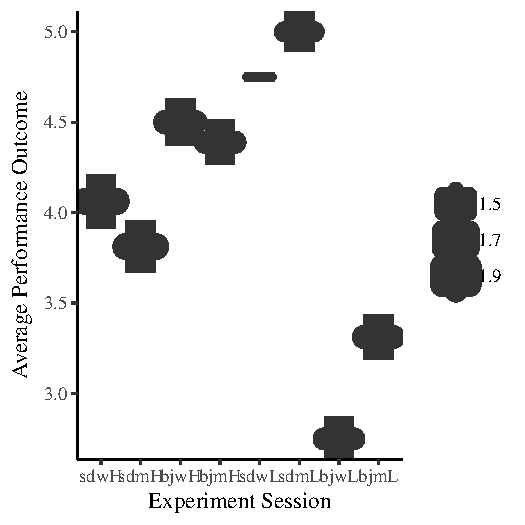
\includegraphics[width=0.5\linewidth,keepaspectratio] {images/fullOutcomeAvgSessionBoxplot-1}
  \label{fig:fullOutcomeAvgSessionBoxplot}
  \caption{Average performance outcome by condition}
\end{figure}

\input{images/ICCtable.tex}

Intra-class correlation estimates were calculated in order to account for the possibility of clustering of model residuals according to groupings of athlete sex, team, experiment location and specific experiment session (see Table ~\ref{tab:ICCTable}). ICC values indicated that between-group variance was low to moderate, with highest values for feelings of group click and social bonding between teams and experimental sessions. Given the constraints on model complexity imposed by the relatively small sample size of the study, experimental session was chosen as a level 2 grouping variable. High variation in the mean and standard deviation of objective performance outcome (see Figure ~\ref{fig:fullOutcomeAvgSessionBoxplot}) further supported the decision to account for variation attributable to experiment session.

Consistent with the previous study, a linear mixed effects regression (LMER) model (package \textit{lme4} in the R environment) was used to test relationships between variables of interest (see Chapter ~\ref{tournamentSurvey} Section ~\ref{survey:survey:dataStructureModelSelection}). To account for clustering within each experimental session, Experiment session was modelled as a random effect (intercept and slope).  Unless otherwise stated, all models controlled for perceptions of individual performance relative to prior expectations, post-Experiment arousal, the average performance outcome of each invasion drill trial, and subjective and objective measures of athlete technical competence, by including these variables as fixed effects.


\myparagraph{Prediction 1: More positive perceptions of team performance relative to prior expectations will correlate with higher feelings of team click with the training group}

\begin{figure}
    \centering
    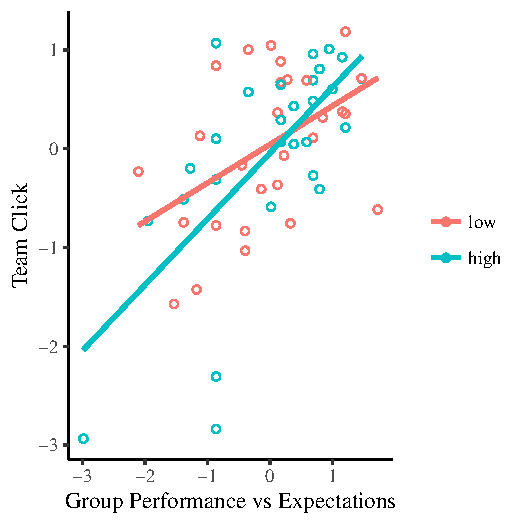
\includegraphics[width=0.5\linewidth,keepaspectratio] {images/teamPerfExpClickScatter-1}
    \caption{More positive perceptions of team performance relative to prior expectations predict group click, moderated by condition ($n = 53$)}
    \label{fig:teamPerfExpClickScatter}
\end{figure}

The relationship between perceptions of group performance relative to prior expectations and group click was modelled using an LMER with group performance expectations, condition, and their interaction included in the model as fixed effects. The model revealed a significant positive interaction effect of group performance expectation violation and condition on group click ($\betavec .41 \CIstart .07, .75 \CIfinish \SE .17, t(53) = 2.39, \pvalue .02 $).  The main effect of condition ($\betavec .76 \CIstart .12, 1.4 \CIfinish \SE .33, t(53) = 2.32, \pvalue .02 $) and group performance expectation violation on feelings of team click with the training group ($\betavec .32 \CIstart .06, .57 \CIfinish, \SE .13, t(53)= 2.41, \pvalue .02$) were also significant.  The average performance outcome of each invasion drill trial was also a significant positive predictor of team click ($\betavec .73 \CIstart .23, 1.24 \CIfinish \SE .26, t(53)= 2.86, \pvalue .006$ (see Table ~\ref{tab:M1lmer}). This result suggested that on-field performance may have influenced athlete perceptions of performance and group click.

These results, visualised in figure ~\ref{fig:teamPerfExpClickScatter}, suggested that perceptions of group performance relative to prior expectations were a positive predictor of feelings of group click among athletes.  This relationship was moderated by experiment condition, such that perceptions of group performance had a greater effect on feelings of group click in the high difficulty condition than in the low difficulty condition.  Model residuals were normally distributed around zero ($\resdist .98, \pvalue .77 $) and an analysis of Cook's distances suggests that the model did not contain any observations that unjustifiably influenced parameter estimates (all $\cooksD < .78$), for full presentation of model assumptions, see Appendix Figure ~\ref{fig:M1Assumptions}).  Results were in line with predictions that more positive perceptions of group performance relative to prior expectations predicted stronger feelings of team click, an effect observed to be strongest in the high difficulty condition.



\myparagraph{Prediction 2: Feelings of group click predict feelings of social bonding to the training group}

\begin{figure}
  \centering
    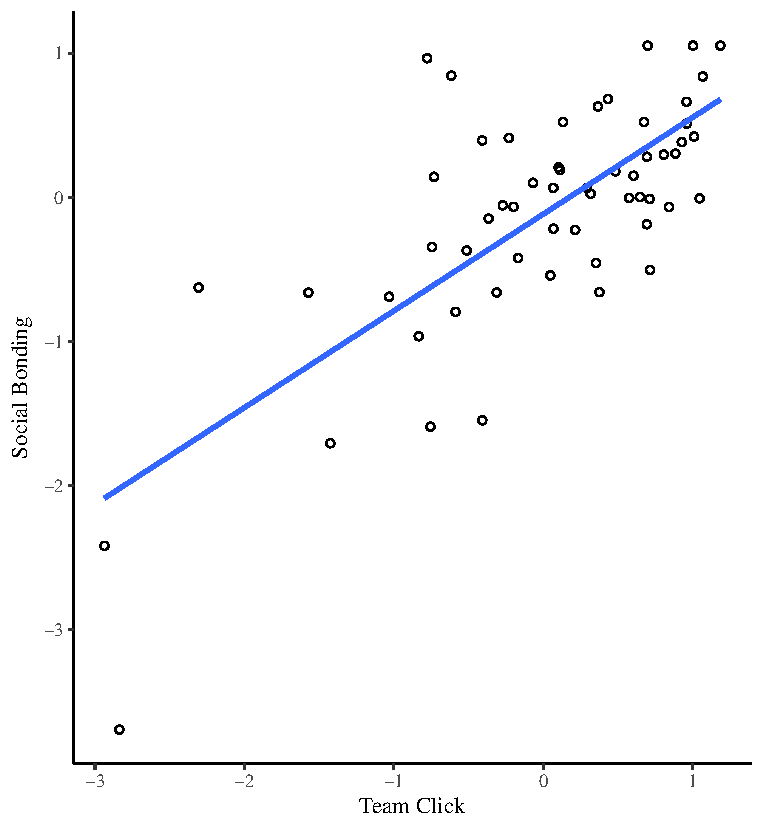
\includegraphics[width=0.5\linewidth,keepaspectratio] {images/groupClickBondScatter}
    \label{fig:groupClickBondScatter}
    \caption{Perceptions of group click predict feelings of social bonding to training group. The interaction effect of condition is not significant ($n = 53$)}
\end{figure}

A LMER model in which group click, condition, and their interaction were included as fixed effects, revealed a strong positive relationship between feelings of group click and feelings of social bonding to the training group, $\betavec .43 \CIstart .15, .72 \CIfinish \SE .14, t(29.22) = 2.96, \pvalue .006, \MR , \CR $.
The main effect of condition ($\betavec .13 \CIstart .15, .72 \CIfinish \SE .29, t(18.7) = 3.15, \pvalue .006$) and the interaction effect of group click and condition on social bonding ($\betavec .26 \CIstart -0.08, .60 \CIfinish \SE .17, t(30.43) = 1.51, \pvalue .14$) were not significant.  These results did, however, appear to be trending in the predicted direction, whereby the relationship between click and bonding appeared stronger in the high difficulty condition.

Figure ~\ref{fig:groupClickBondScatter} represents the results of the model.  These results suggesting that athletes who felt stronger levels of group click also felt stronger levels of social bonding to their training group, irrespective of experiment condition.  Model residuals were normally distributed around zero ($\resdist .99, \pvalue .96$) and there were no unjustifiably influential cases (all $\cooksD < .79$, see model assumptions in Figure ~\ref{fig:M2Assumptions} of Appendix ~\ref{app6:trainingExperiment} Section ~\ref{app6:postExperimentModelAssumptions}).







\myparagraph{Prediction 3: More positive violations of team performance expectations will predict higher levels of social bonding to the training group}

\begin{figure}
  \centering
  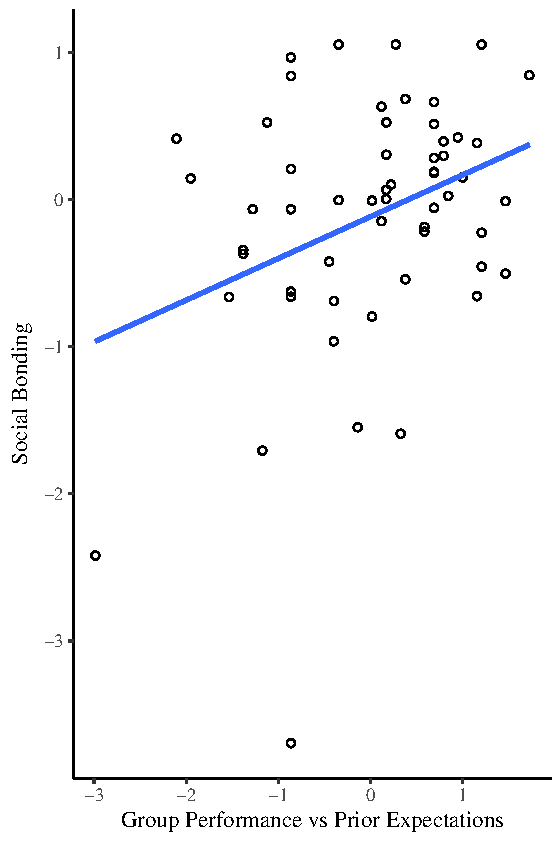
\includegraphics[width=0.5\linewidth,keepaspectratio] {images/groupPerfExpBondConditionScatter}
  \caption{Positive violation of group performance expectations
 predict feelings of social bonding to training group}
 \label{fig:groupPerfExpBondConditionScatter}
\end{figure}

A LMER model revealed a significant positive interaction of perceptions of group performance relative to prior expectations and condition on social bonding, $\betavec .46 \CIstart .10, .82 \CIfinish \SE .18, t(53) = 2.5, \pvalue .02, \MR , \CR $.  Average performance in each trial was also a significant predictor of social bonding, $\betavec .65 \CIstart .11, 1.19 \CIfinish \SE .27, t(53) = 2.37, \pvalue .02$.
The main effects of group performance vs expectations ($\betavec .008  \CIstart -.27, .28 \CIfinish \SE .14, t(53) = .06, \pvalue .96$) and condition ($\betavec .56  \CIstart 1.12, 1.25 \CIfinish \SE .35, t(53) = 1.6, \pvalue .11$) were not significant. The result for the fixed effect of condition did, however, appear to be trending in the predicted direction ($p = .11$). These results indicate that the the relationship between group performance expectations vs expectations and social bonding was significant only in the high difficulty condition, as demonstrated visually in figure ~\ref{fig:groupPerfExpBondConditionScatter}.
Model residuals were normally distributed around zero ($\resdist .97, \pvalue .31, and all \cooksD < .55$, see model assumptions in Appendix  ~\ref{fig:M3Assumptions}).  These results suggested that the relationship between positive violation of group performance expectations and social bonding was significant, only in the high difficulty condition, and not overall across conditions.









\myparagraph{Prediction 4: Feelings of group click will mediate a relationship between more positive violations of expectations around group performance and social bonding to the group}


Mediation analyses were conducted using linear mixed effects regressions in the Causal Mediation Analysis package in R (Version 4.4.5).  To make inferences concerning the average indirect and total effects, quasi-Bayesian Markov Chain Monte Carlo (MCMC) method based on normal approximation and 1000 simulations was used to estimate the 95\% Confidence Intervals \citep{Tofighi2016a,Imai2010}. MCMC estimation is a form of non-parametric bootstrapping whereby the sampling distribution for the effect of interest is not assumed to be normal but is instead simulated from the model estimates and their asymptotic variances and covariances \cite{Preacher2008}.

\begin{figure}
  \centering
  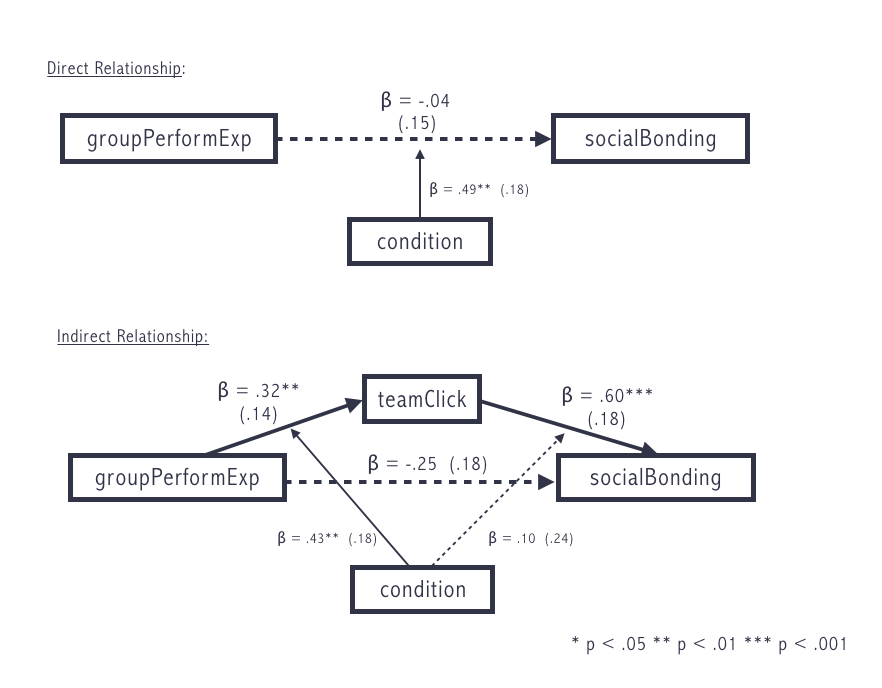
\includegraphics[width=0.9\linewidth,keepaspectratio] {images/postExperimentModMedFigure}
  \caption{Partial moderated mediation model: group click mediates the realtionship between group performance and social bonding.  This effect is partially moderated by condition (high).}
  \label{fig:postExperimentModMedFigure}
\end{figure}

\begin{figure}
  \centering
  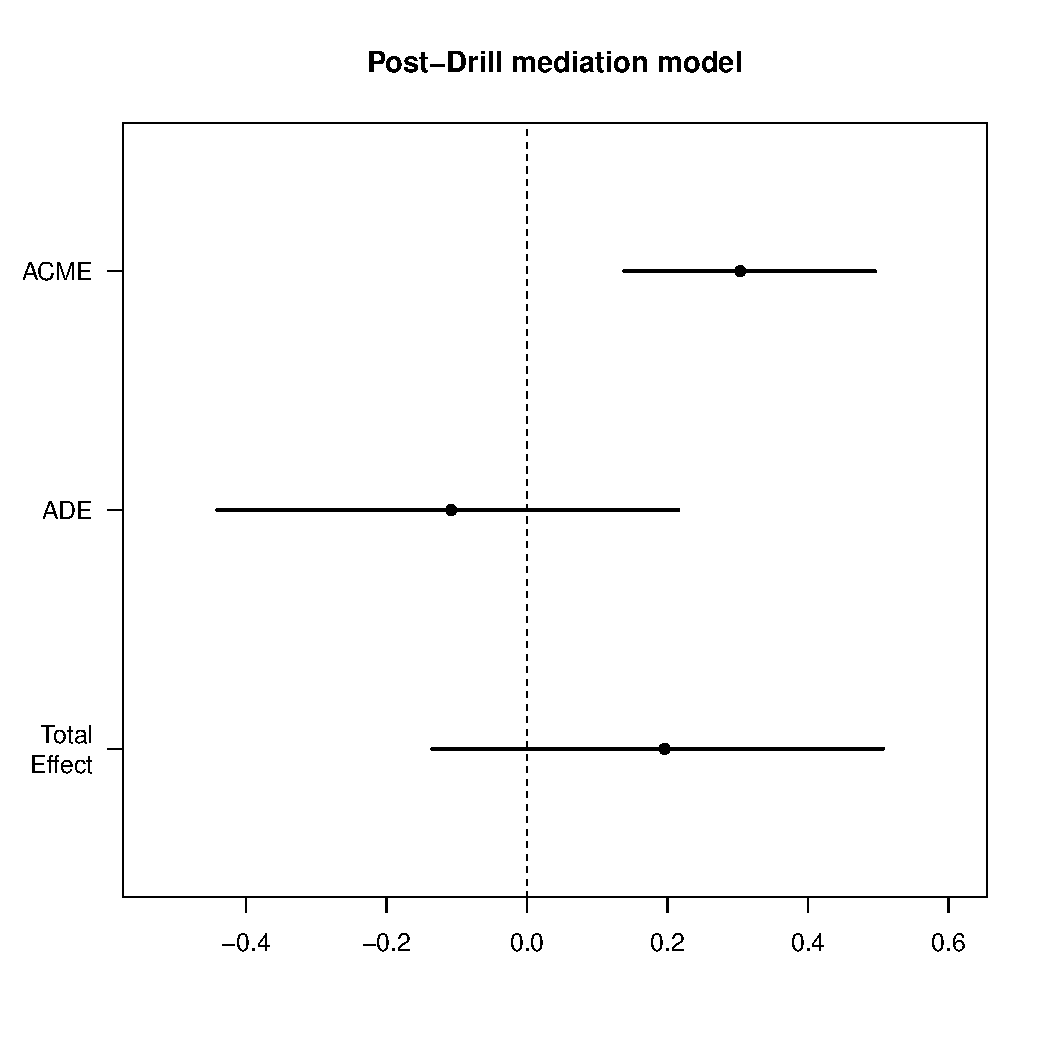
\includegraphics[width=0.5\linewidth,keepaspectratio] {images/groupPerfExpClickMediationPlot}
  \caption{Change in group click fully mediates relationship between team performance expectation violation and social bonding. ACME = Average conditional mediation effect; ADE = Average direct effect.}
  \label{fig:groupPerfExpClickChangeMedPlot}
\end{figure}


\begin{figure}
  \centering
  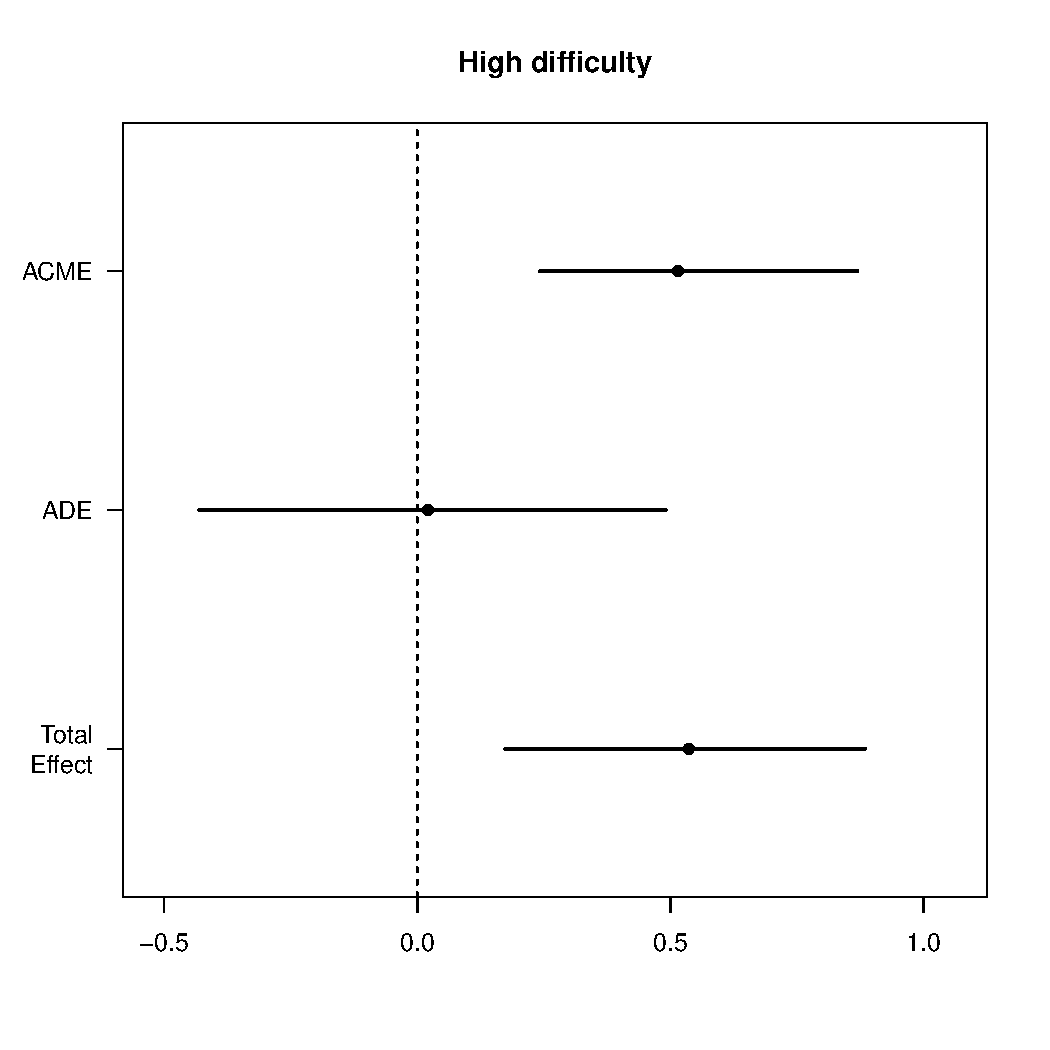
\includegraphics[width=0.5\linewidth,keepaspectratio] {images/groupPerfExpClickMediationPlotHigh}
  \caption{Change in group click mediates relationship between change in group performance expectation violation and change in group bonding in the High condition}
  \label{fig:groupPerfClickChangeMedPlotHigh}
\end{figure}

\begin{figure}
  \centering
  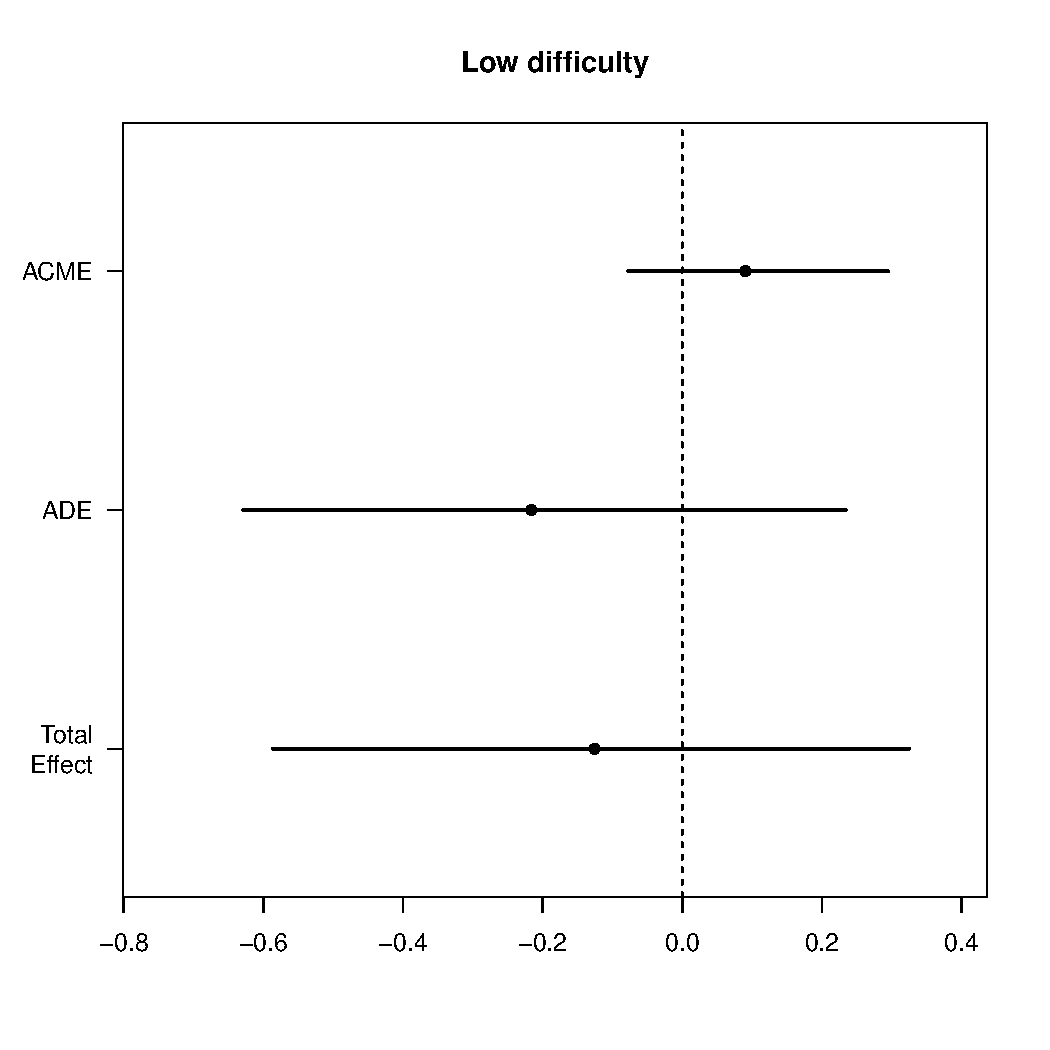
\includegraphics[width=0.5\linewidth,keepaspectratio] {images/groupPerfExpClickMediationPlotLow}
  \caption{Change in group click mediates relationship between change in group performance expectation violation and change in group bonding, but not in the Low condition.}
  \label{fig:groupPerfClickChangeMedPlotLow}
\end{figure}







\myparagraph{Summary of post-Experiment results}

Post-Experiment generally confirmed predictions by demonstrating positive significant associations between perceptions of performance (relative to prior expectations), group click, and social bonding.  The mediation effect also confirmed that the experience of high quality coordination in joint action (team click) mediated a relationship between joint action and social bonding.  The fact that this result was further moderated by experiment condition suggests that (positive) expectation violation in joint action could be an important explanatory mechanism.  The moderation effect of condition was only significant in the relationship between group performance vs. expectations and team click, however.











\subsection{Analysis of Pre-post Experiment Survey Data}

Analysis of pre- to post-Experiment change in variables of interest followed the same procedure as the post-Tournament analysis.


\newgeometry{margin=0.5cm} % modify this if you need even more space
  \begin{landscape}
    \centering
      % latex table generated in R 3.5.0 by xtable 1.8-2 package
% Mon Aug 27 19:27:29 2018
\begin{table}[ht]
\centering
\begin{tabular}{rlll}
  \hline
 & Baseline & Pre & Post \\ 
  \hline
n &    58 &    58 &    58 \\ 
  JointActionSuccess (mean (sd)) &   NaN (NA) &  0.27 (0.86) & -0.28 (1.01) \\ 
  IndividualComponentPerformance (mean (sd)) & -0.05 (0.98) &  0.10 (0.93) & -0.06 (0.97) \\ 
  GroupPerformVsExpected (mean (sd)) &   NaN (NA) &   NaN (NA) & 63.37 (21.23) \\ 
  IndividualPerformanceExpectations (mean (sd)) &   NaN (NA) &   NaN (NA) & 61.49 (17.44) \\ 
  GroupClick (mean (sd)) &   NaN (NA) &  0.19 (0.85) & -0.19 (0.97) \\ 
  GroupBonding (mean (sd)) &   NaN (NA) &  0.12 (0.81) & -0.12 (0.85) \\ 
  GroupClickPost (mean (sd)) &   NaN (NA) &   NaN (NA) & -0.00 (0.93) \\ 
  TeamBondingFactor (mean (sd)) &  0.02 (0.93) &   NaN (NA) & -0.02 (0.84) \\ 
  Arousal (mean (sd)) &   NaN (NA) & -0.23 (0.94) &  0.23 (0.92) \\ 
   \hline
\end{tabular}
\caption{Variables of interest over time 
 for entire sample} 
\label{tab:factorsTime}
\end{table}

   \end{landscape}
\restoregeometry

Table ~\ref{tab:factorsTime} shows that the post-Experiment measures of Joint Action Success and group click were significantly lower than pre-Experiment measurements.  In fact, it appeared that the mean of almost all key variables of interest decreased in value between pre- and post-Experiment measurements. One exception was physiological arousal, which significantly increased following the experiment, as would be expected due to the moderate to high levels of physiological exertion associated with the training drill.  Athlete perceptions of components of individual performance and bonding to the team as a whole did not vary significantly across time points.



\subsubsection{Pre-Post Experiment variation in variables of interest by condition}

Figures ~\ref{fig:groupPerfConfPlot}\nobreakdash~\ref{fig:prePostBondingPlot} in Appendix ~\ref{app6:trainingExperiment} Section ~\ref{app6:conditionDifferencesPrePost} contrast pre-post variation in key variables of interest according to experiment condition. LMER was used to model the relationship between condition and variation in key variables of interest (group performance, click, and bonding) over time. Owing to the repeated measures structure of the data, individual athlete was included with and experiment session as random a intercept (slopes were not modelled due to insufficient sample size), and time, condition, and their interaction were included as main effects. Models revealed significant main effects of time (Pre-Post Experiment) on group performance relative to prior expectations ($\betavec -.66 \CIstart -1.14, -.17 \CIfinish \SE .24, t(115) = -2.67, \pvalue .008 $), group click, ($\betavec -.44 \CIstart -.76, -.12 \CIfinish \SE .16, t(58.19) = -2.69, \pvalue .009 $) or group bonding ($\betavec -.20 \CIstart -.40, -.01 \CIfinish \SE .10, t(56.91) = -2.07, \pvalue .04$), but no significant main effects of condition on group performance relative to prior expectations ($\betavec .36 \CIstart -1.27, 2.09 \CIfinish \SE .88, t(115) = .41, \pvalue .68$), group click, ($\betavec -.18 \CIstart -1.45, 1.10 \CIfinish \SE .65, t(59.44) = -.27, \pvalue .79 $) or group bonding ($\betavec .42 \CIstart -.44, 1.28 \CIfinish \SE .44, t(37.23) = .97, \pvalue .34$).
Interaction effects were also not significant for group performance relative to prior expectations ($\betavec -.11 \CIstart -.79, .57 \CIfinish \SE .35, t(115) = -.33, \pvalue .74 $), group click, ($\betavec .12 \CIstart -.34, .57 \CIfinish \SE .23, t(57.81) = .50, \pvalue .62$) or group bonding ($\betavec -.09 \CIstart -.37, .18 \CIfinish \SE .14, t(56.73) = -.68, \pvalue .50$).

These results suggested that there was no obvious variation by condition over time---at least in the current structure of the data in which significant decreases in variables over time may have drowned out any significant increases in variables pre- to post-Experiment.

\myparagraph{Construction of new variables expressing change in variables over time (pre- to post-Experiment)}

To find evidence for predicted positive associations between variables within a larger trend in which mean values of most measures decreased between pre- to post-Experiment, new variables were created which expressed each individual athlete's change in reports relating to performance, group click, and social bonding between two time points.  Values at time 1 (pre-Experiment) were subtracted from values at time 2 (post-Experiment) and created as a new variable.  Relationships between these new variables (change in group performance vs expectations, change in group click, change in group bonding) were used to analyse study predictions.



\myparagraph{Model Structure}
For the LMER models that follow, as in the previous section, experimental session was identified as a group-level variable in the multi-level structure, based on an assessment of ICC values between main variables of interest (see Table ~\ref{app6:modelSelectionPrePost} in Appendix ~\ref{app6:trainingExperiment} Section ~\ref{app6:modelSelectionPrePost}).



\myparagraph{Prediction 1: More positive change in group performance vs expectations will correlate with higher change in feelings of group click with the training group}

\begin{figure}
    \centering
    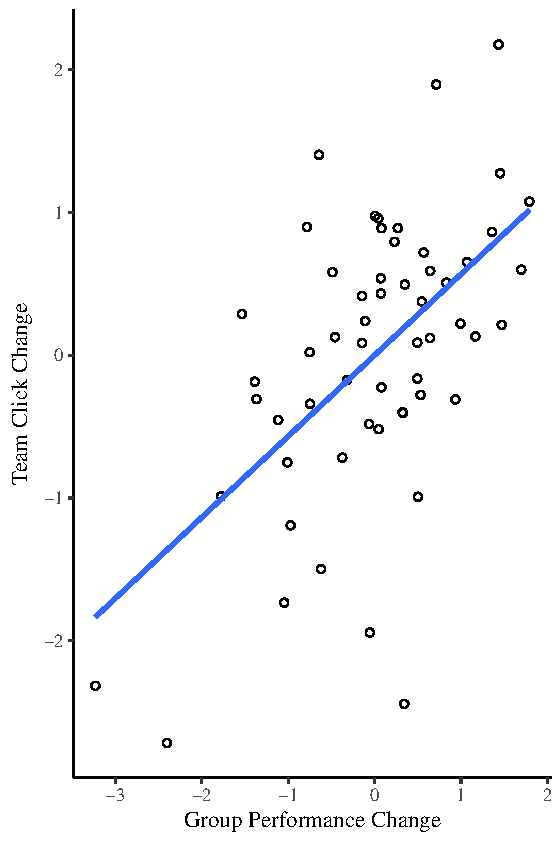
\includegraphics[width=0.5\linewidth,keepaspectratio] {images/groupPerfClickChangeCondition}
    \caption{Change in group performance predicts change in group click, moderated by condition ($n = 53$)}
    \label{fig:groupPerfClickChangeCondition}
\end{figure}

An LMER, with change in perceptions of group performance, condition, and their interaction included in the model as fixed effects, revealed a significant positive interaction effect of group performance vs expectations and condition on group click
($\betavec .49 \CIstart .06, .92 \CIfinish \SE .22, t(53) = 2.22, \pvalue .03 \MR \CR $).
The main effect of change in group performance expectation on change in group click was also (highly) significant, ($\betavec .76 \CIstart .46, 1.06 \CIfinish \SE .15, t(53) = 5.018, \pvalue .00006 $). The main effect of condition, however, was not significant ($\betavec .08 \CIstart -.69, .85 \CIfinish \SE .39, t(53) = .20, \pvalue .84 $).
These results---visualised in figure ~\ref{fig:groupPerfClickChangeCondition}---suggested that change in perceptions of group performance were a positive predictor of increase in feelings of group click following the experiment.  This relationship is moderated by condition, such that athletes in the high difficulty condition showed a higher increase than athletes in the low difficulty condition.

Model residuals were normally distributed around zero ($\resdist .98, \pvalue .45$) and an analysis of Cook's distances suggests that the model did not contain any observations that unjustifiably influenced parameter estimates (all $\cooksD < .34$), for full presentation of model assumptions, see Appendix Figure ~\ref{fig:M1PrePostAssumptions}).





\myparagraph{Prediction 2: Change in group click predicts change in feelings of social bonding to the training group}

\begin{figure}
  \centering
    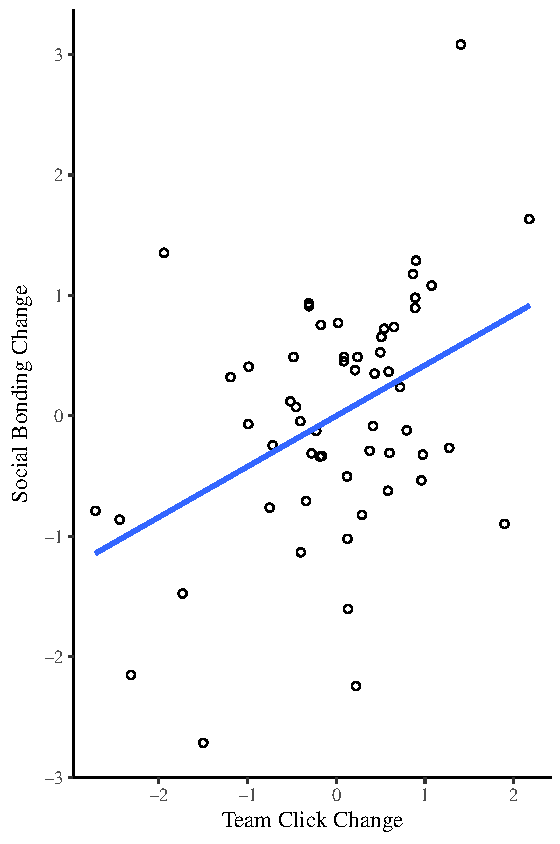
\includegraphics[width=0.5\linewidth,keepaspectratio] {images/groupClickBondingChangeCondition}
    \label{fig:groupClickBondingChangeCondition}
    \caption{Change in perceptions of group click predict change in feelings of social bonding to training group, moderated by condition ($n = 53$)}
\end{figure}

A LMER model revealed a significant interaction effect of change in group click and experiment condition on change social bonding, ($\betavec .76 \CIstart .32, 1.19 \CIfinish \SE.22, t(47.05) = 3.41, \pvalue .001, \MR , \CR $).  The main effect of change in group click was also a significant predictor of change in social bonding, ($\betavec .58 \CIstart .32, .84 \CIfinish \SE.13, t(40.03) = 4.36, p < .0001 $).  The main effect of condition was not significant, ($\betavec .03 \CIstart -.79, .84 \CIfinish \SE.41, t(17.66) = .06, p < .95 $).  A scatter plot shows that the relationship between change in group click and change in bonding is most pronounced in the high difficulty condition (see figure ~\ref{fig:groupClickBondingChangeCondition}). These results suggest that athletes who felt stronger levels of group click also felt stronger levels of social bonding to their training group, irrespective of experiment condition.

Model residuals were not normally distributed around zero ($\resdist .93, \pvalue .006$). Based on an Cook's Distances, the model did not appear to contain any observations that unjustifiably influenced parameter estimates (all $\cooksD < .49$), but the distribution of residuals and QQ PLot did show a clear positive outlier (for full presentation of model assumptions, see Figure ~\ref{fig:M22Assumptions} in Appendix ~\ref{app6:trainingExperiment} Section ~\ref{app6:prePostExperimentModelAssumptions}).





\myparagraph{Prediction 3: More positive perceptions of team performance relative to prior expectations will predict higher levels of social bonding to the training group}

\begin{figure}
  \centering
  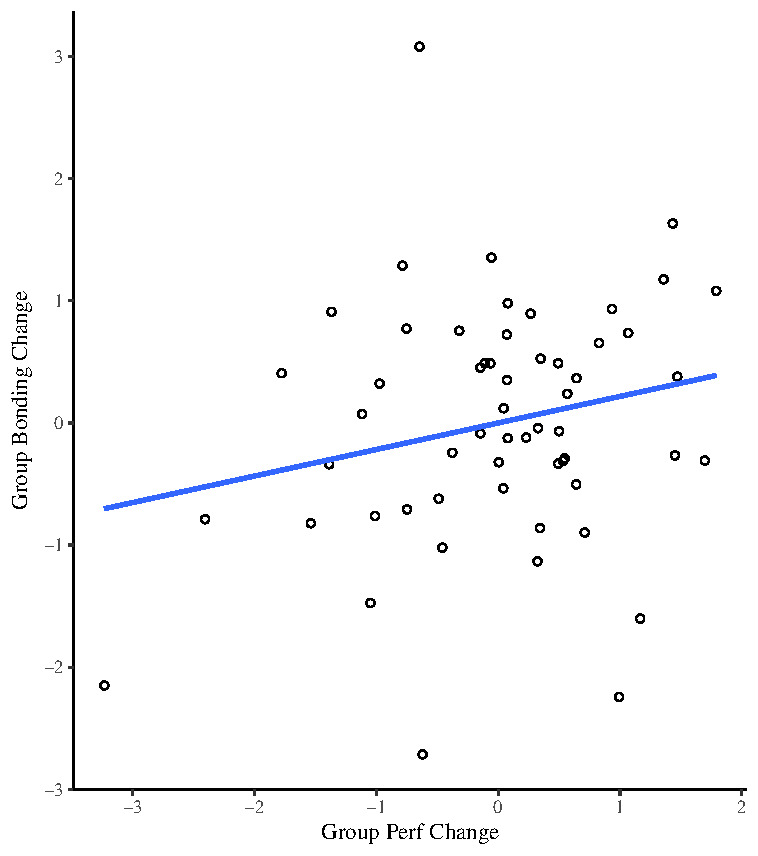
\includegraphics[width=0.5\linewidth,keepaspectratio] {images/groupPerfBondingChangeCondition}
  \caption{Change in perceptions of group performance predict change in social bonding to the training group, moderated by condition ($n = 53$)}
 \label{fig:groupPerfBondingChangeCondition}
\end{figure}

The interaction effect of change in perceptions of group performance and condition significantly predicted variation in change in social bonding, ($\betavec .49 \CIstart .46, 1.38  \CIfinish \SE .53, t(53) = 4.03, \pvalue .0001, \MR , \CR $). The main effect of change in group performance was also significant, ($\betavec .21  \CIstart .16, .78 \CIfinish \SE.23, t(53) = 2.33, \pvalue .02$), as was the main effect of change in perceptions of individual performance, ($\betavec .26  \CIstart .02, .50 \CIfinish \SE.12, t(53) = 2.15, \pvalue .04$).
For a full report of model statistics, see APPENDIX ~\ref{tab:M2PrePostOutput}.  This model suggested that the relationship between group performance expectations vs expectations and social bonding was significant only in the high difficulty condition, as demonstrated visually in figure ~\ref{fig:groupPerfExpBondConditionScatter}.

Model residuals were normally distributed around zero (\resdist .97, \pvalue .31) and all $\cooksD < .22$, see figure ~\ref{fig:M23Assumptions} Appendix ~\ref{app6:trainingExperiment}).  These results suggested that the relationship between  group performance vs expectations and social bonding was significant, only in the high difficulty condition, and not overall across conditions. For a full report on tests of model assumptions, see APPENDIX ~\ref{fig:M23Assumptions}.







\myparagraph{Prediction 4: Change in feelings of group click will mediate a relationship between more positive change in perceptions of  group performance and social bonding to the group}






Procedure for mediation analyses were consistent with the post-Tournament analysis (see Section ~\ref{}, subsection ~\ref{} HYPERLINK).

Results of the mediation analysis revealed significant average indirect effect of change in group performance perception on change in social social bonding, attributable to change in group click, $\betavec.09 \CIstart .10, .02  \CIfinish, \pvalue .02$.  When controlling for the effect of group click on social bonding, the average direct effect between Joint Action Success and social bonding was no longer significant, $\betavec -.08  \CIstart -.23, .06 \CIfinish, \pvalue .24$  (see Figure ~\ref{fig:groupPerfExpClickMediationPlot}).

Closer analysis revealed that the mediation was moderated by experiment condition: the mediation was significant only for the high difficulty condition ($\betavec .52  \CIstart .24, .87 \CIfinish, p <=.0001$), but not the low difficulty condition, ($\betavec .09  \CIstart -.08, .30 \CIfinish, p =.32$). The moderated mediation model is shown in figure ~\ref{fig:prePostExperimentChangeModMedFigure}, and the overall and moderated mediation effects are contrasted graphically in figures ~\ref{fig:groupPerfExpClickChangeMedPlot}\nobreakdash~\ref{fig:prePostExperimentChangePlotLow}.  These results suggest that feelings of group click fully mediate the relationship between change in perceptions of group performance and social bonding, only in the high experiment condition.  In a similar fashion to the results of the post-Experiment analysis, results supported predictions that feelings of group click fully mediate a relationship between experience of social bonding and social bonding.

\begin{figure}
  \centering
  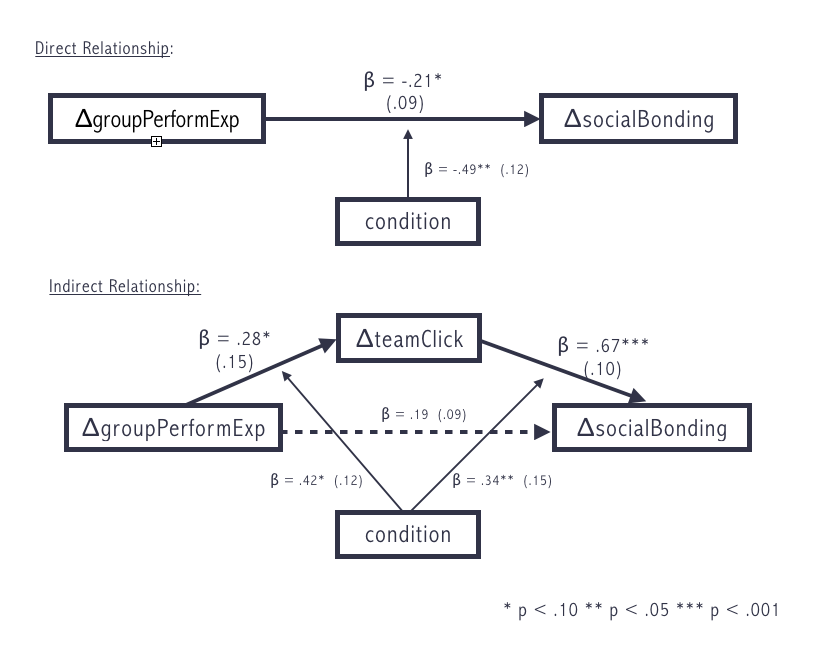
\includegraphics[width=0.9\linewidth,keepaspectratio] {images/prePostExperimentChangeModMedFigure}
  \caption{Moderated mediation model: group click mediates the realtionship between group performance and social bonding.  This effect is partially moderated by condition (high).}
  \label{fig:prePostExperimentChangeModMedFigure}
\end{figure}

\begin{figure}
  \centering
  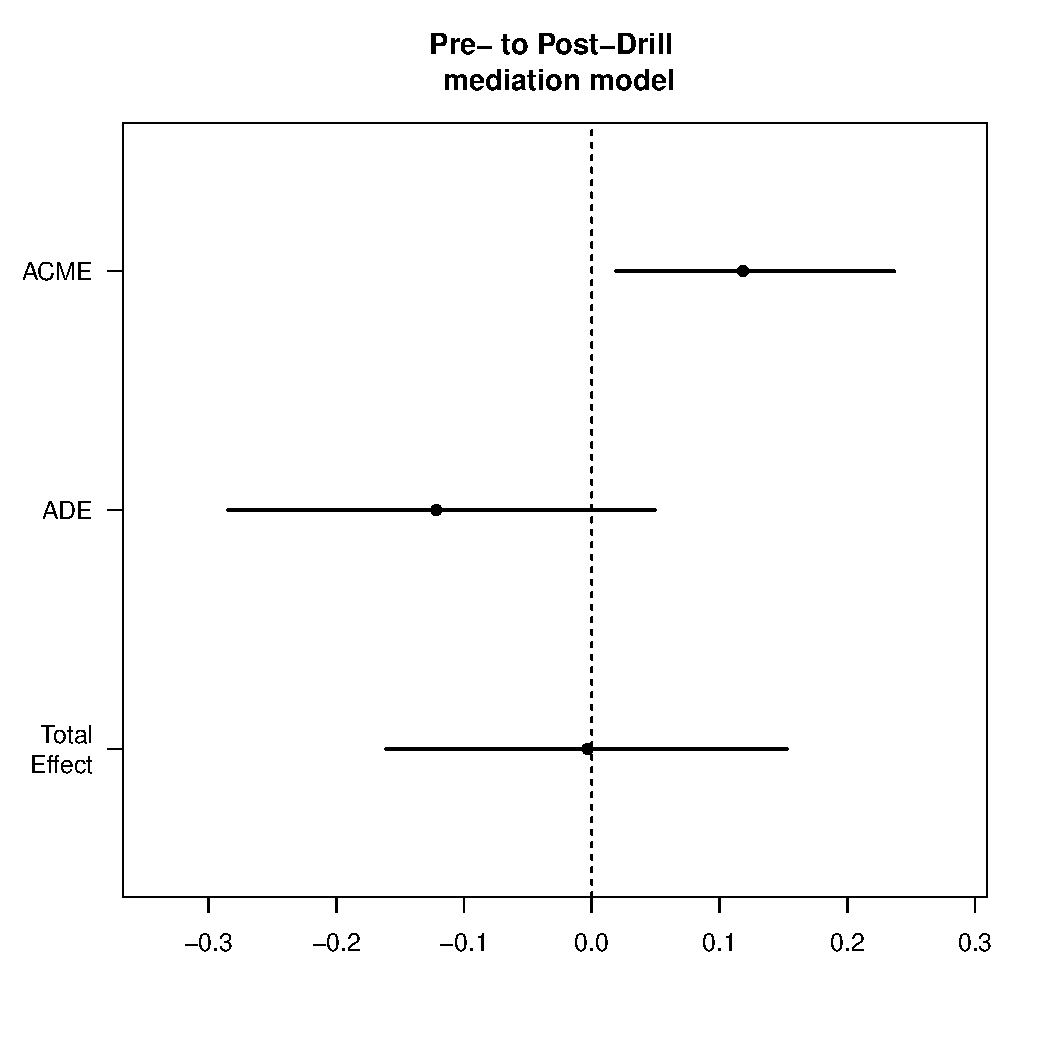
\includegraphics[width=0.5\linewidth,keepaspectratio] {images/groupPerfExpClickChangeMedPlot}
  \caption{Group click partially mediates relationship between group performance vs expectation and social bonding}
  \label{fig:groupPerfExpClickChangeMedPlot}
\end{figure}

\begin{figure}
  \centering
  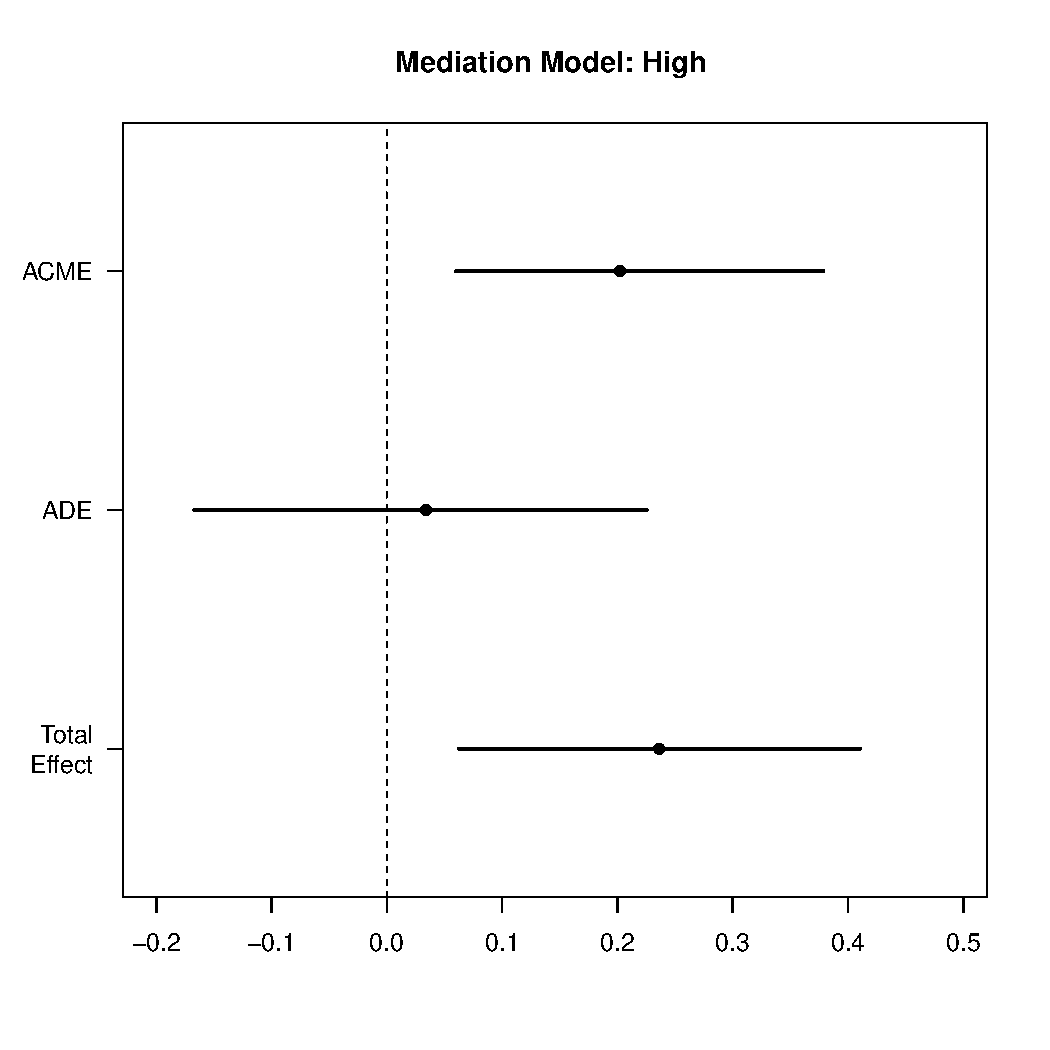
\includegraphics[width=0.5\linewidth,keepaspectratio] {images/groupPerfClickChangeMedPlotHigh}
  \caption{Change in group click partially mediates relationship between group performance and social bonding}
  \label{fig:groupPerfClickChangeMedPlotHigh}
\end{figure}

\begin{figure}
  \centering
  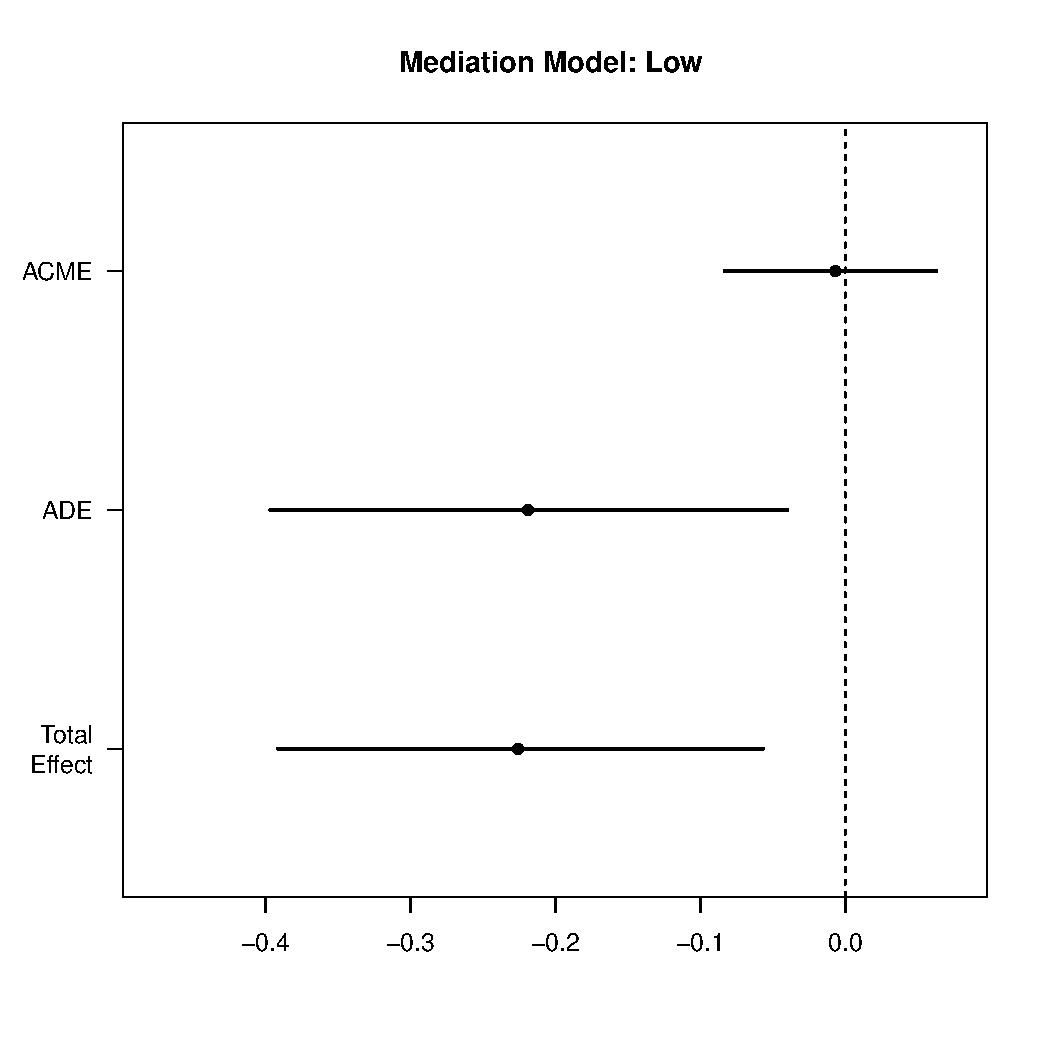
\includegraphics[width=0.5\linewidth,keepaspectratio] {images/groupPerfClickChangeMedPlotLow}
  \caption{Group click partially mediates relationship between group performance and social bonding}
  \label{fig:prePostExperimentChangePlotLow}
\end{figure}





\section{Discussion of Results}
%study:
This study was designed to investigate the social cognition of team click in a controlled field experiment.  Athletes participated in a training drill paradigm in which overt feedback concerning performance was restricted to athletes' perceptions of each phase of the invasion drill.  Athletes were not overtly declared as winners or losers, and there was nothing explicit to gain from the experiment---unlike in the high stakes national tournament that was the focus of the previous study (Chapter ~\ref{tournamentSurvey}).  Unlike a high stakes rugby tournament, the training drill did not entail high levels of physiological cost, in fact only required low-to-medium level exertion and ``grab'' as opposed to full-contact. Instead, coordination in joint action was isolated as the key component of the experimental paradigm.  Results of this study generally support study predictions, and reproduced the correlational results of the survey study in a more controlled setting. Taken toghether, these empirical studies substantiate ethnographic observations made in the first part of this dissertation, and offer preliminary evidence for a novel theory, outlined in this thesis, of social bonding through joint action in group exercise contexts.

%results:
Significant positive relationships between 1) perceptions of performance in joint action relative to prior expectation and team click, 2) team click and social bonding,  and 3) performance in joint action and social bonding were moderated by experiment condition, such that these relationships were strongest in athletes who participated in the high difficulty condition.  Mediation models supported these findings, showing evidence of a moderated mediation effect of team click on the relationship between group performance vs expectations and social bonding.  In both the post-Experiment and pre- to post-Experiment analyses, the mediation effect was moderated by experiment condition: the relationship was either strongest or only present in the high difficulty condition on not in the low difficulty condition.  Despite an overall trend in which scores decreased between pre- and post-Experiment measures, athletes who on average experienced more positive perceptions of performance following the Experiment also reported higher average levels of team click and social bonding (a statistical relationship that was against the overall trend in the data).  The results described here held when statistically controlling for athlete perceptions of individual performance, technical competence, objective performance outcome in the experiment session, and physiological arousal.

%inferences
From these results it is possible to infer that perceptions of joint action feature strongly in athletes' formulation of social attitudes, for example feelings of social bonding and group membership.  The experience of higher levels of click in joint action may also be a particularly powerful phenomenon in the formation of positive associations with teammates and team identity.  In addition, results of this study provide some support for the theory, outlined in this dissertations, that the formulation and violation of expectations around joint action is a mechanism of central importance to the social cognition of joint action.  The exhilarating phenomenon of team click in joint action could be associated with positive violations of athletes expectations, which are implicitly formulated and calibrated over time with their teammates in training and competition.  Interactive team sports such as rugby provide a situation in which optimising quality of joint action is the explicit shared goal of the group---the group's reason for being----and so it is understandable that joint action would feature strongly in athlete inferences about group membership.


%limitations
Although the experiment manipulation appeared to statistically moderate a relationship between joint action and social bonding, these results were not supported by the study's manipulation checks, all of which did not produce significant results.  The design and execution of the experiment was such that the possibility that the significant moderating effect of condition was the artefact of low sample size and limited randomisation of athlete sampling. The experiment manipulation was subtle, and was delivered by a researcher who spoke Chinese as a second language, perhaps unable to manufacture a sufficient performance pre-Experiment to alter the expectations of athletes. In addition, the limitations of research context, namely time constraints and access to athletes, were such that pilot phase was not exhaustive as it could have been (2 trials per condition).

The experiment sought to isolate expectation violation as a mechanism of central importance to the social cognition of joint action.  While results show evidence for condition-wise effects, in which the high difficulty condition was responsible for moderating the relationship between joint action, team click, and social bonding, it is not sufficiently clear precisely what mechanism drove these results.
The fact that the hypothesised mechanisms of joint action and social bonding have been shown to exist pre-declaratively and predominantly below the surface of conscious experience presents a methodological challenge for psychological research which relies heavily on self-report.

Further exploring the relationship between pre-perceptual regulatory mechanisms of joint action and their psychosocial effects will require the use of other methods of data collection and analysis in order to triangulate the reliability of self-report data \citep{Newell2014}.  In this specific example, motion capture from video footage allows for measuring synchrony between co-actors could using both traditional methods of dimension reduction and principal component analysis \citep[see for example][]{Riley2011} as well as emerging methods borrowed from dynamic systems theory including fractal-like 1/f scaling (``pink noise'') \citep[see for example][]{Holden2013}. It is quite possible that these different measurements of synchrony could access different psychophysiological dimensions of the relationship between joint action and social bonding.  Other physiological markers of social interaction such as heart rate variability \citep{Konvalinka2011,Fischer2014a} and pain threshold \citep{Cohen2009,Tarr2015}) are beginning to be developed and tested in both experimental and real-world settings.
These novel methodological approaches help complement existing behavioural measures, such as such as economic games \citep{Xygalatas2013} and spontaneous helping tasks \citep{Kirschner2010}, designed to access psychological mechanisms related to social bonding and cooperation.
Together, these measures could then be compared to self-report measures derived from athlete self-report to more fully understand the ways in which component mechanisms and system dynamics of joint action generate social cohesion \citep{Marsh2009}.



%    [ ] what inferences can we make from these results?
%    [ ] How does it relate to other literature?
%    [ ] limitations
%    [ ] future work —> experiment (takes away explicit feedback)
%    [ ]  "Conclude the general discussion with a strong paragraph stating the main point or points again, in somewhat different terms-if possible-than used before.”
